% Options for packages loaded elsewhere
\PassOptionsToPackage{unicode}{hyperref}
\PassOptionsToPackage{hyphens}{url}
%
\documentclass[
]{book}
\usepackage{lmodern}
\usepackage{amssymb,amsmath}
\usepackage{ifxetex,ifluatex}
\ifnum 0\ifxetex 1\fi\ifluatex 1\fi=0 % if pdftex
  \usepackage[T1]{fontenc}
  \usepackage[utf8]{inputenc}
  \usepackage{textcomp} % provide euro and other symbols
\else % if luatex or xetex
  \usepackage{unicode-math}
  \defaultfontfeatures{Scale=MatchLowercase}
  \defaultfontfeatures[\rmfamily]{Ligatures=TeX,Scale=1}
\fi
% Use upquote if available, for straight quotes in verbatim environments
\IfFileExists{upquote.sty}{\usepackage{upquote}}{}
\IfFileExists{microtype.sty}{% use microtype if available
  \usepackage[]{microtype}
  \UseMicrotypeSet[protrusion]{basicmath} % disable protrusion for tt fonts
}{}
\makeatletter
\@ifundefined{KOMAClassName}{% if non-KOMA class
  \IfFileExists{parskip.sty}{%
    \usepackage{parskip}
  }{% else
    \setlength{\parindent}{0pt}
    \setlength{\parskip}{6pt plus 2pt minus 1pt}}
}{% if KOMA class
  \KOMAoptions{parskip=half}}
\makeatother
\usepackage{xcolor}
\IfFileExists{xurl.sty}{\usepackage{xurl}}{} % add URL line breaks if available
\IfFileExists{bookmark.sty}{\usepackage{bookmark}}{\usepackage{hyperref}}
\hypersetup{
  pdftitle={EBM \& Statistiek III},
  pdfauthor={Robby.DePauw@Ugent.be},
  hidelinks,
  pdfcreator={LaTeX via pandoc}}
\urlstyle{same} % disable monospaced font for URLs
\usepackage{color}
\usepackage{fancyvrb}
\newcommand{\VerbBar}{|}
\newcommand{\VERB}{\Verb[commandchars=\\\{\}]}
\DefineVerbatimEnvironment{Highlighting}{Verbatim}{commandchars=\\\{\}}
% Add ',fontsize=\small' for more characters per line
\usepackage{framed}
\definecolor{shadecolor}{RGB}{248,248,248}
\newenvironment{Shaded}{\begin{snugshade}}{\end{snugshade}}
\newcommand{\AlertTok}[1]{\textcolor[rgb]{0.94,0.16,0.16}{#1}}
\newcommand{\AnnotationTok}[1]{\textcolor[rgb]{0.56,0.35,0.01}{\textbf{\textit{#1}}}}
\newcommand{\AttributeTok}[1]{\textcolor[rgb]{0.77,0.63,0.00}{#1}}
\newcommand{\BaseNTok}[1]{\textcolor[rgb]{0.00,0.00,0.81}{#1}}
\newcommand{\BuiltInTok}[1]{#1}
\newcommand{\CharTok}[1]{\textcolor[rgb]{0.31,0.60,0.02}{#1}}
\newcommand{\CommentTok}[1]{\textcolor[rgb]{0.56,0.35,0.01}{\textit{#1}}}
\newcommand{\CommentVarTok}[1]{\textcolor[rgb]{0.56,0.35,0.01}{\textbf{\textit{#1}}}}
\newcommand{\ConstantTok}[1]{\textcolor[rgb]{0.00,0.00,0.00}{#1}}
\newcommand{\ControlFlowTok}[1]{\textcolor[rgb]{0.13,0.29,0.53}{\textbf{#1}}}
\newcommand{\DataTypeTok}[1]{\textcolor[rgb]{0.13,0.29,0.53}{#1}}
\newcommand{\DecValTok}[1]{\textcolor[rgb]{0.00,0.00,0.81}{#1}}
\newcommand{\DocumentationTok}[1]{\textcolor[rgb]{0.56,0.35,0.01}{\textbf{\textit{#1}}}}
\newcommand{\ErrorTok}[1]{\textcolor[rgb]{0.64,0.00,0.00}{\textbf{#1}}}
\newcommand{\ExtensionTok}[1]{#1}
\newcommand{\FloatTok}[1]{\textcolor[rgb]{0.00,0.00,0.81}{#1}}
\newcommand{\FunctionTok}[1]{\textcolor[rgb]{0.00,0.00,0.00}{#1}}
\newcommand{\ImportTok}[1]{#1}
\newcommand{\InformationTok}[1]{\textcolor[rgb]{0.56,0.35,0.01}{\textbf{\textit{#1}}}}
\newcommand{\KeywordTok}[1]{\textcolor[rgb]{0.13,0.29,0.53}{\textbf{#1}}}
\newcommand{\NormalTok}[1]{#1}
\newcommand{\OperatorTok}[1]{\textcolor[rgb]{0.81,0.36,0.00}{\textbf{#1}}}
\newcommand{\OtherTok}[1]{\textcolor[rgb]{0.56,0.35,0.01}{#1}}
\newcommand{\PreprocessorTok}[1]{\textcolor[rgb]{0.56,0.35,0.01}{\textit{#1}}}
\newcommand{\RegionMarkerTok}[1]{#1}
\newcommand{\SpecialCharTok}[1]{\textcolor[rgb]{0.00,0.00,0.00}{#1}}
\newcommand{\SpecialStringTok}[1]{\textcolor[rgb]{0.31,0.60,0.02}{#1}}
\newcommand{\StringTok}[1]{\textcolor[rgb]{0.31,0.60,0.02}{#1}}
\newcommand{\VariableTok}[1]{\textcolor[rgb]{0.00,0.00,0.00}{#1}}
\newcommand{\VerbatimStringTok}[1]{\textcolor[rgb]{0.31,0.60,0.02}{#1}}
\newcommand{\WarningTok}[1]{\textcolor[rgb]{0.56,0.35,0.01}{\textbf{\textit{#1}}}}
\usepackage{longtable,booktabs}
% Correct order of tables after \paragraph or \subparagraph
\usepackage{etoolbox}
\makeatletter
\patchcmd\longtable{\par}{\if@noskipsec\mbox{}\fi\par}{}{}
\makeatother
% Allow footnotes in longtable head/foot
\IfFileExists{footnotehyper.sty}{\usepackage{footnotehyper}}{\usepackage{footnote}}
\makesavenoteenv{longtable}
\usepackage{graphicx,grffile}
\makeatletter
\def\maxwidth{\ifdim\Gin@nat@width>\linewidth\linewidth\else\Gin@nat@width\fi}
\def\maxheight{\ifdim\Gin@nat@height>\textheight\textheight\else\Gin@nat@height\fi}
\makeatother
% Scale images if necessary, so that they will not overflow the page
% margins by default, and it is still possible to overwrite the defaults
% using explicit options in \includegraphics[width, height, ...]{}
\setkeys{Gin}{width=\maxwidth,height=\maxheight,keepaspectratio}
% Set default figure placement to htbp
\makeatletter
\def\fps@figure{htbp}
\makeatother
\setlength{\emergencystretch}{3em} % prevent overfull lines
\providecommand{\tightlist}{%
  \setlength{\itemsep}{0pt}\setlength{\parskip}{0pt}}
\setcounter{secnumdepth}{5}
\mainmatter

\title{EBM \& Statistiek III}
\author{\href{mailto:Robby.DePauw@Ugent.be}{\nolinkurl{Robby.DePauw@Ugent.be}}}
\date{2021-11-08}

\usepackage{amsthm}
\newtheorem{theorem}{Theorem}[chapter]
\newtheorem{lemma}{Lemma}[chapter]
\newtheorem{corollary}{Corollary}[chapter]
\newtheorem{proposition}{Proposition}[chapter]
\newtheorem{conjecture}{Conjecture}[chapter]
\theoremstyle{definition}
\newtheorem{definition}{Definition}[chapter]
\theoremstyle{definition}
\newtheorem{example}{Example}[chapter]
\theoremstyle{definition}
\newtheorem{exercise}{Exercise}[chapter]
\theoremstyle{definition}
\newtheorem{hypothesis}{Hypothesis}[chapter]
\theoremstyle{remark}
\newtheorem*{remark}{Remark}
\newtheorem*{solution}{Solution}
\begin{document}
\maketitle

{
\setcounter{tocdepth}{2}
\tableofcontents
}
\hypertarget{over-deze-cursus}{%
\chapter*{Over deze cursus}\label{over-deze-cursus}}


De cursus {EBM \& Statistiek III} bouwt verder op de leerstof uit {EBM \& Statistiek I} en {EBM \& Statistiek II}. De situering, vereiste begincompetanties en eindcompetenties zijn terug te vinden op de vak-specifieke pagina op \href{https://ufora.ugent.be}{Ufora}. Binnen deze cursus bespreken we meer geavanceerde statistische modellen. De belangrijkste van deze modellen zijn:

\begin{itemize}
\tightlist
\item
  Bivariate correlaties
\item
  Lineaire regressie
\item
  Logistische regressie
\item
  Mixed models
\item
  Overlevingsanalyses
\end{itemize}

Binnen deze cursus maken we gebruik van enkele oefeningen in {SPSS}


\includegraphics[width=1.04167in,height=\textheight]{img/spss.png}

Probeer voor de oefeningen versie 26 van {SPSS} te gebruiken indien deze beschikbaar is op Athena. Er kan ook steeds een stand-alone versie van {SPSS} aangevraagd worden via volgende \href{https://helpdesk.ugent.be/athena/}{link}. \textbf{Opgelet}: de website met instructies om {SPSS} te installeren op jouw computer is alleen beschikbaar vanuit het UGent netwerk of via VPN.

\hypertarget{de-lesgever}{%
\section*{De lesgever}\label{de-lesgever}}


De lessen binnen het vak worden georganiseerd door \emph{dr. Robby De Pauw} en \emph{prof. dr. Pascal Coorevits}. Vragen kunnen steeds gepost worden in de discussieruimtes op Ufora.

Voor vragen over het stuk statistiek kunnen jullie steeds mailen naar \href{mailto:Robby.DePauw@Ugent.be}{\nolinkurl{Robby.DePauw@Ugent.be}}, voor vragen over het stuk datamanegement kunnen jullie mailen naar \href{mailto:Pascal.Coorevits@Ugent.be}{\nolinkurl{Pascal.Coorevits@Ugent.be}}.

\hypertarget{uiprintversie-boek}{%
\section*{Uiprintversie boek}\label{uiprintversie-boek}}


Bovenaan de balk van deze website kunnen jullie een pdf-versie van dit boek downloaden.

\begin{Shaded}
\begin{Highlighting}[]
\NormalTok{knitr}\OperatorTok{::}\KeywordTok{asis_output}\NormalTok{(}\StringTok{'}\CharTok{\textbackslash{}\textbackslash{}}\StringTok{mainmatter}\CharTok{\textbackslash{}n\textbackslash{}n}\StringTok{'}\NormalTok{)}
\end{Highlighting}
\end{Shaded}

\mainmatter

\hypertarget{intro}{%
\chapter{Introductie}\label{intro}}

Het onderzoekproces bestaat uit verschillende belnagrijke stappen die nodig zijn om tot een duidelijk en rechtlijnige conclusie te komen. In de voorbije jaren hebben jullie de verschillende onderzoekstappen bestudeerd en zijn jullie geëindig met één van de laatste stappen van het onderzoeksproces, de \textbf{inductieve statistiek}. Enkele kernbegrippen hierbij waren \emph{hypothese}, \emph{fouten} bij hypothesetesten en statistische \emph{toetsen}. Hieronder bespreken we kort deze belangrijke concepten opnieuw. Voor meer informatie verwijzen we naar de cursussen uit {EBM \& Statistiek I} en {EBM \& Statistiek II}.

\hypertarget{hypothesetoetsen}{%
\section*{Hypothesetoetsen}\label{hypothesetoetsen}}


Een hypothesetoets bestaat uit twee delen, de nulhypothese \(H_0\) en de alternatieve hypothese \(H_1\) of \(H_a\). De aanvaarde methode is dat men voorlopig aanneemt dat het effect niet bestaat, en nagaat of deze veronderstelling stand kan houden in het licht van de verzamelde. De veronderstelling dat ene effect (verschil, associatie, \ldots) niet bestaan is dan ook vaak het uitgangspunt binnen \(H_0\). Op basis van de verzamelde data proberen we \(H_0\) te verwerpen in het voordeel van \(H_a\). De beslissing om \(H_0\) te verwerpen gebeurt uiteindelijk op basis van de \(p\)-waarde. Als cut-off punt wordt hier vaak 5\% (of 0.05) genomen. We noemen deze ciut-off waarde ook wel het significantieniveau of \(\alpha\) Waarom specifiek deze cut-off gebruikt wordt, wordt uitgelegd in het volgende deel van de cursus.

Aangenomen wordt dat geen effect geassocieerd wordt met \(H_0\), wat niet betekend dat er geen a:ternatieve mogelijk zijn. We kunnen bijvoorbeeld ook stellen dat we onder \(H_O\) veronderstellen dat een effect een specifiek getal moet zijn.

\hypertarget{fouten-bij-hypothesetoetsen}{%
\section*{Fouten bij hypothesetoetsen}\label{fouten-bij-hypothesetoetsen}}


Op basis van een hypothesetoetse die we uitvoeren op basis van verzamelde data uit een steekproef van een bepaalde populatie proberen we een besluit te vormen over de hypothese binnen de populatie. Aangezien een steekproef en metingen gepaard gaan met variabiliteit en onzekerheid, kunnen er fouten optreden. In onderstaande tabel vinden jullie een grafische weergave van deze mogelijke fouten:

\begin{Shaded}
\begin{Highlighting}[]
\NormalTok{knitr}\OperatorTok{::}\NormalTok{opts_chunk}\OperatorTok{$}\KeywordTok{set}\NormalTok{(}\DataTypeTok{echo =} \OtherTok{FALSE}\NormalTok{, }\DataTypeTok{message =} \OtherTok{FALSE}\NormalTok{, }\DataTypeTok{warning =} \OtherTok{FALSE}\NormalTok{)}
\end{Highlighting}
\end{Shaded}

\begin{figure}
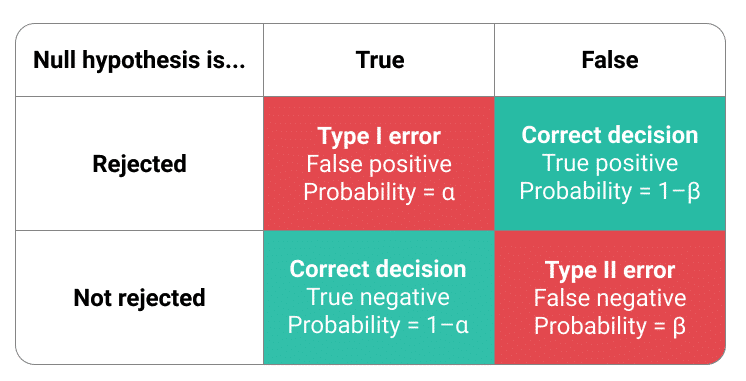
\includegraphics[width=0.9\linewidth]{img/error} \caption{Visuele samenvatting van fouten bij hypothesetoetsen.}\label{fig:error}
\end{figure}

\textbf{Voorbeeld:} Veronderstel dat er binnen de populatie van kinesitherapeuten geen verschil is in het aantal uren die gepresteerd worden tussen mannen en vrouwen. We organiseren binnen deze populatie (\(n = 30\)) en evaluaeren het aantal uren. Uiteindelijk voeren we een statistische toets uit, waaruit we finaal besluiten of er al dan geen verschil is in gepresteerde uren. Hiervoor veronderstellen we volgende hypothesen:

\begin{itemize}
\tightlist
\item
  \(H_0\): Er is geen verschil in gepresteerde uren tussen mannen en vrouwen.
\item
  \(H_1\): Er is een verschil in gepresteerde uren tussen mannen en vrouwen.
\end{itemize}

Indien we binnen de populatie weten dat er \textbf{geen} verschil is (\(H_0\) is dus juist), zijn er twee mogelijke uitkomsten:

\begin{itemize}
\tightlist
\item
  We verwerpen \(H_0\) en besluiten dus dat er wel een verschil is. In dit scenario maken we een fout en binnen de inductieve statistiek wordt deze fout aangeduid als \(\alpha\) (Type I error). Algemeen wordt aanvaard om deze \(\alpha\) op 5\% te zetten.
\item
  We aanvaarden \(H_0\) en besluiten dus dat er wel een verschil is. In dit scenario maken we een correcte beslissing.
\end{itemize}

Indien we binnen de populatie weten dat er \textbf{wel} verschil is (\(H_0\) is dus fout), zijn er twee mogelijke uitkomsten:

\begin{itemize}
\tightlist
\item
  We verwerpen \(H_0\) en besluiten dus dat er wel een verschil is. In dit scenario maken we een correcte beslissing.
\item
  We aanvaarden \(H_0\) en besluiten dus dat er geen verschil is. In dit scenario maken we een fout en binnen de inductieve statistiek wordt deze fout aangeduid als \(\beta\) (Type II error). Over de grootte van \(\beta\) is er minder consensus, maar 80\% wordt vaak algemeen aanvaard.
\end{itemize}

In bovenstaande figuur \ref{fig:error} kan je de \textbf{vier} verschillende scenario's zoals hierboven beschreven herkennen.

\hypertarget{keuze-statistische-toets}{%
\section*{Keuze statistische toets}\label{keuze-statistische-toets}}


In figuur \ref{fig:stattest} vinden jullie een schema met de specifieke keuze van statistische toets op basis van de gestelde voorwaarden.

\begin{figure}
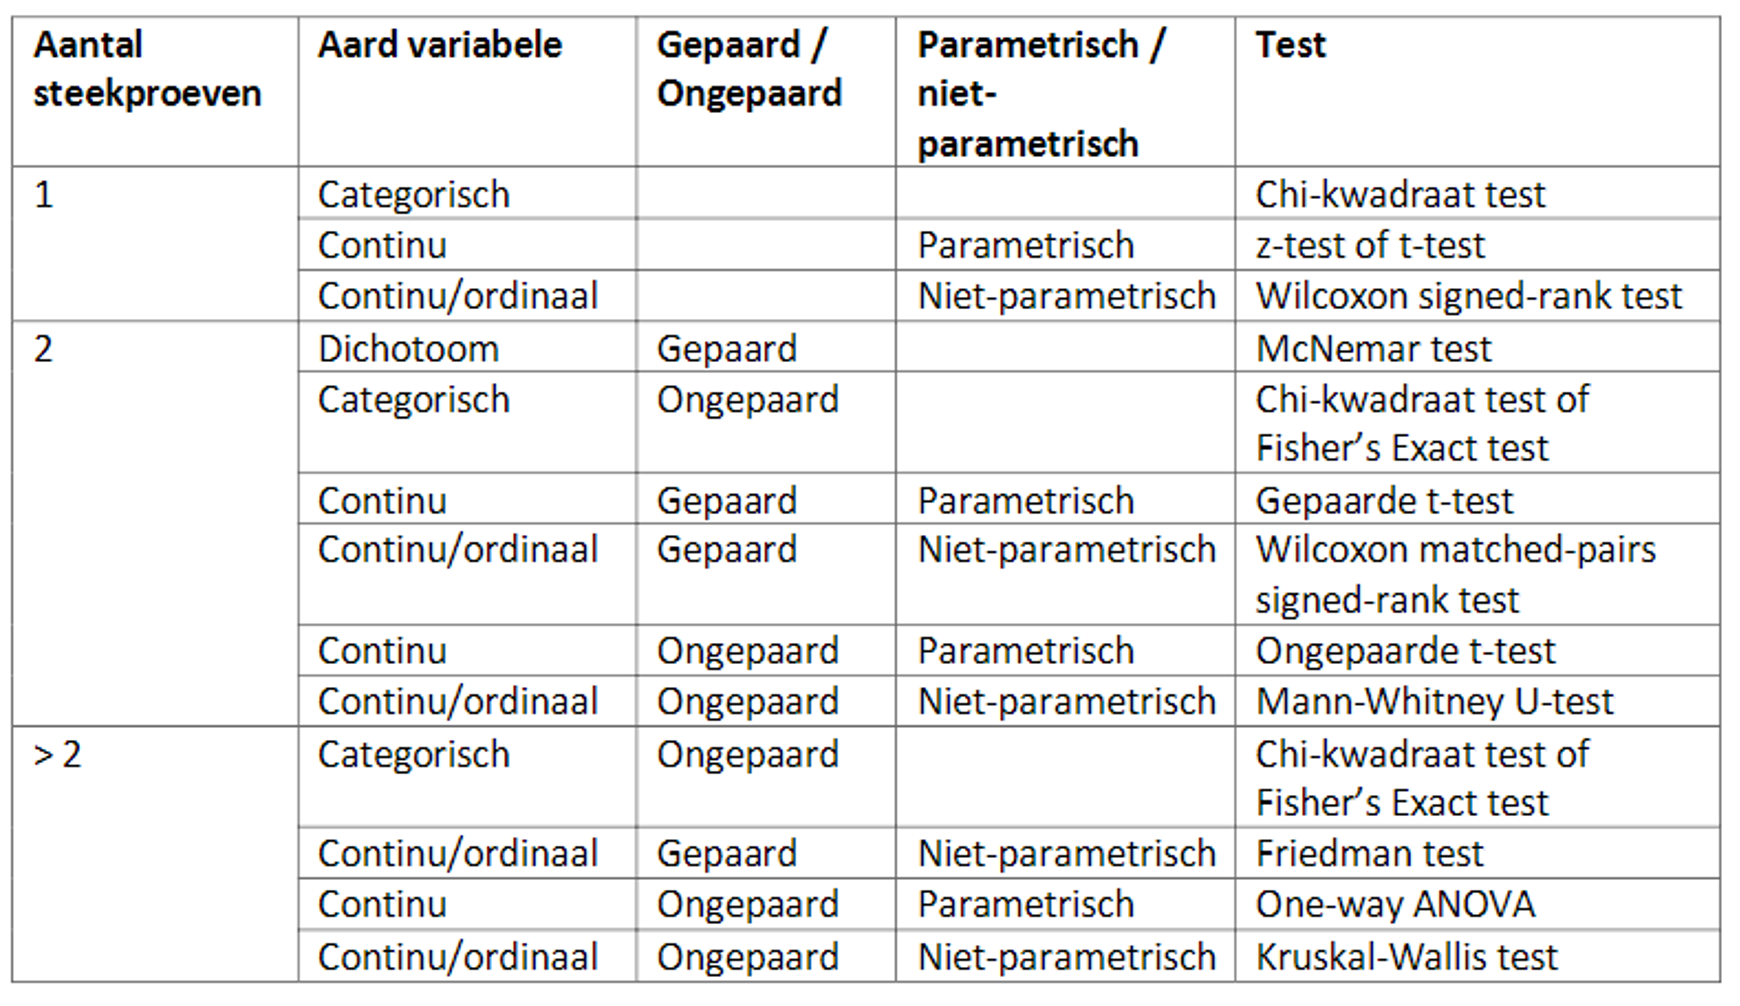
\includegraphics[width=1\linewidth]{img/stat_test} \caption{Keuze van statistische toetsen.}\label{fig:stattest}
\end{figure}

\mainmatter

\hypertarget{corr}{%
\chapter{Correlaties}\label{corr}}

In de paper van Al-Hadidi et al.~(2019) vermeld men volgende stelling:

\begin{quote}
``A significant positive correlation was also found between the duration of use for studying and the duration of pain (p\textless{} 0.001, r = 0.212).''

---Al-Hadidi et al.~(2019)
\end{quote}

\begin{itemize}
\tightlist
\item
  Kunnen we hieruit besluiten dat verhoogd smartphonegebruik de oorzaak is van langdurigere nekpijnervaringen?
\item
  Hoe interpreteren we de \(r\) en \(p\)-waarde? Kunnen we hieruit besluiten dat er een sterke link is?
\end{itemize}

\hypertarget{inleiding}{%
\section*{Inleiding}\label{inleiding}}


Er zijn verschillende manieren om een associatie tussen twee variabelen in te schatten. Eén van de meest gebruikte statistische maten om een verband tussen twee variabelen aan te tonen is een correlatie. Er is er een uitgebreid gamma aan correlaties beschikbaar die gebruikt worden om een verband tussen verschillende specifieke types variabelen aan te tonen. Binnen deze cursus focussen we op correlatiecoëfficiënten die het verband tussen twee \textbf{continue} variabelen trachten in te schatten.

Belangrijk om te onthouden is dat correlaties nooit een oorzaak-gevolg relatie kunnen inschatten binnen een cross-sectionele studie. Oorzaak-gevolg relaties (of causale relaties) kunnen enkel aangetoond worden bij gerandomiseerde studies (vb. RCT). Dit is één van de voornaamste redenen waarom een RCT bovenaan de evidentietabellen terug te vinden is (Figuur \ref{fig:evidenceladder}). Binnen een niet-gerandomiseerde studie kan een schatting van de correlatie vervuild/verstoord zijn door onderliggen de factoren die een belangrijke rol spelen, maar niet in rekening werden gebracht of niet geobserveerd werden.

\begin{figure}
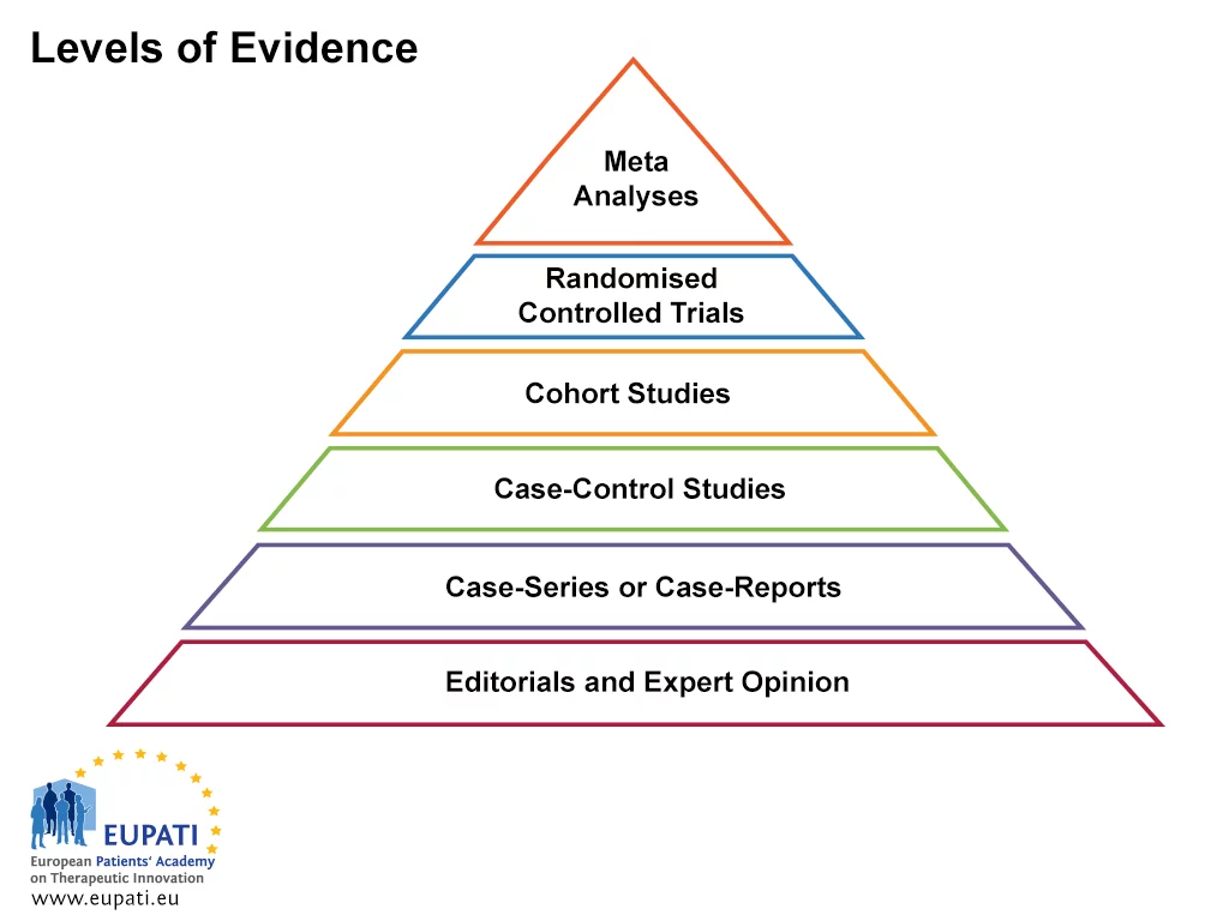
\includegraphics[width=1\linewidth]{img/evidenceladder} \caption{Evidentiepiramide.}\label{fig:evidenceladder}
\end{figure}

Volgend voorbeeld verduidelijkt het probleem van vervuilig van een associatie. In tabel \ref{tab:aggr}, worden de resultaten weergegeven van deze studie. Zoals aangegeven in deze tabel is het slaagpercentage 80\% binnen de groep van mannen en is het slaagpercentage 67\% binnen de groep van vrouwen. Hieruit zouden we kunnen besluiten dat er significant minder vrouwen slagen op een wiskundetoets in vergelijking met mannen.

\begin{table}

\caption{\label{tab:aggr}Scores op wiskundetoets bij studenten na behalen diploma per geslacht.}
\centering
\begin{tabular}[t]{lrr}
\toprule
Gender & Geslaagd & Niet Geslaagd\\
\midrule
Man & 40 & 10\\
Vrouw & 20 & 10\\
\bottomrule
\end{tabular}
\end{table}

Wanneer we echter kijken naar de slaagpercentages per studie-achtergrond (Tabel \ref{tab:aggr}), dan blijkt het slaagpercentage in elke groep hetzelfde te zijn. Binnen de groep van wiskundestudenten slaagt iedereen (100\%) en binnen de groep van studenten met een achtergrond binnen de psychologie slaagt 50\%. De vervuiling van de associatie, waardoor het lijkt dat de slaagpercentages hoger zijn bij mannen in vergelijking met vrouwen, treedt op wanneer we geen rekening houden met de studie-achtergrond van de studenten. Dit is een type-voorbeeld van het optreden van \textbf{confounding} binnen een studie.

\begin{table}

\caption{\label{tab:cond}Scores op wiskundetoets bij studenten na behalen diploma per geslacht en achtergrond.}
\centering
\begin{tabular}[t]{llrr}
\toprule
Faculty & Gender & Geslaagd & Niet Geslaagd\\
\midrule
Wiskunde & Man & 30 & 0\\
Wiskunde & Vrouw & 10 & 0\\
Psychologie & Man & 10 & 10\\
Psychologie & Vrouw & 10 & 10\\
\bottomrule
\end{tabular}
\end{table}

\textbf{Een correlatie} geeft binnen een cross-sectionele studie nooit een causaal verband weer. Er kunnen steeds andere factoren onrechtstreeks betrokken zijn die ertoe leiden dat er een correlatie tussen twee variabelen ontstaat, zonder dat dit verband effectief aanwezig is.

\hypertarget{soorten-correlaties}{%
\section*{Soorten correlaties}\label{soorten-correlaties}}


Een veelgebruikte maat voor het beschrijven van een associatie tussen twee variabelen is een correlatie. Een correlatie is een schatting die de sterkte van het verband weergeeft tussen twee variabelen en de kan variëreren tussen \(-1\) en \(1\) (\(\rho \in [-1, 1]\)). Wanneer een correlatie dicht bij \(0\) ligt, wijst dit om geen associatie tussen twee variabelen, terwijl een correlatie dicht bij \(\pm 1\), wijst op een sterk verband tussen twee variabelen. In dedze cursus worden twee correlaties besproken, de Pearson correlatie coëfficiënt (\(\rho\)) en de Spearman correlatie coëfficiënt (\(r_s\)), die elk een specifiek verband weergeven.

\begin{figure}
\centering
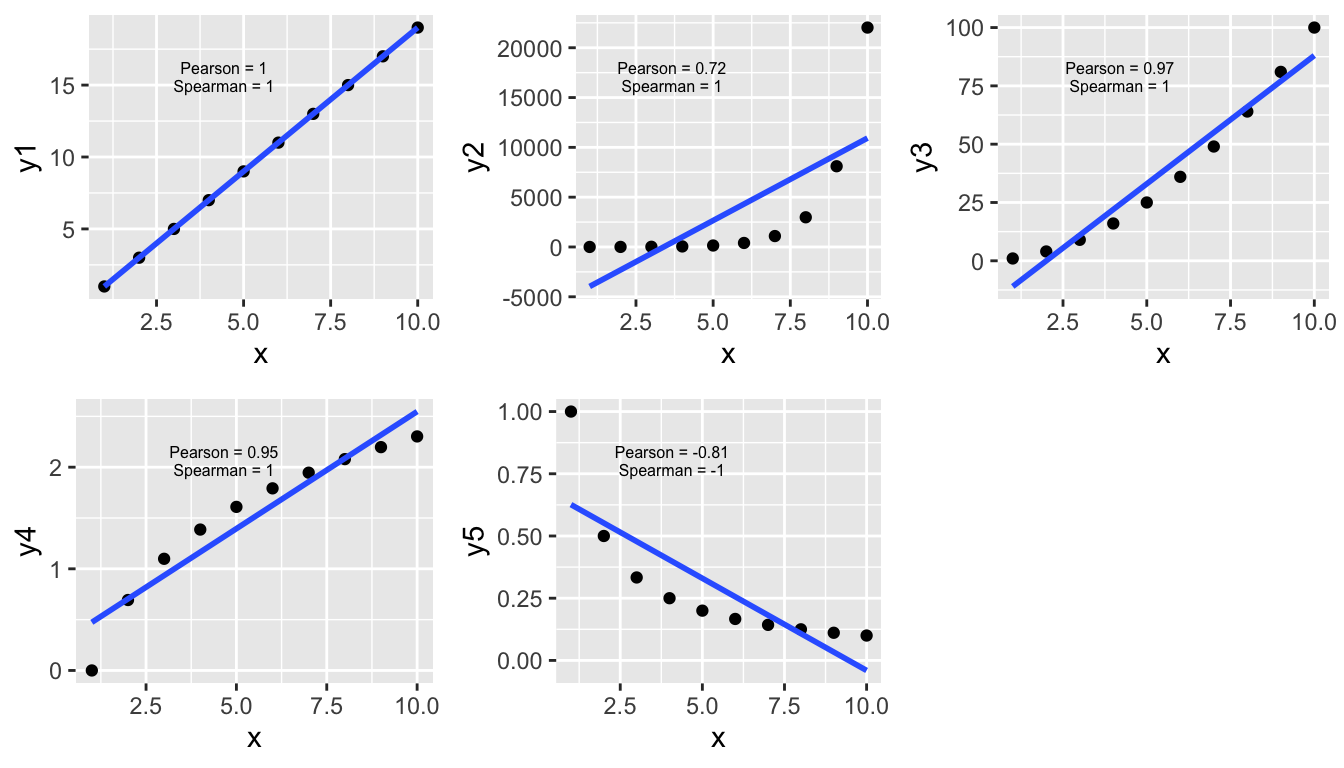
\includegraphics{ugent-ebmstatIII_files/figure-latex/corrs-1.pdf}
\caption{\label{fig:corrs}Different types of associations and their respective correlations}
\end{figure}

In figuur \ref{fig:corrs}, staan een aantal correlaties weergegeven. In deze figuur worden een aantal spreidingsdiagrammen weergegeven waarbij de relatie tussen \(X\) en \(Y\) steeds verschillend is. De punten op de grafiek geven de effectieve waarden weer voor elke observatie, die men kan weergeven als punt (\(x_i\), \(y_i\)). De blauwe lijn op de grafiek geeft steeds de best passende rechte weer door de puntenwolk. Het valt op dat elke Spearman correlatie (\(r_s\)) gelijk is aan 1 of -1 en de Pearson correlatie varieert. Dit fenomeen kan je als volgt interpreteren: een Pearson correlatie het lineaire of rechtlijnige verband nagaat tussen twee variabelen, terwijl de Spearman correlatie nagaat of het om een monotone relatie gaat. Een monotone relatie is een relatie waarbij bij een toename van \(X\), ofwel \(Y\) altijd toeneemt ofwel \(Y\) altijd afneemt. De eerste 4 figuren geven een positief verband weer en ook een positieve correlatie, waarbij een toename in \(X\) samengaat met een toename in \(Y\). De laatste figuur geeft een negatieve relatie weer, waarbij een toename in \(X\) samengaat met een afname in \(Y\).

\begin{table}

\caption{\label{tab:corrtab}Overzicht van karakteristieken en eigenschappen van correlaties.}
\centering
\begin{tabular}[t]{lll}
\toprule
Karakteristieken & Pearson correlatie & Spearman correlatie\\
\midrule
Voorwaarde & Normaal verdeling beide variabelen & Geen\\
Soort relatie & Lineaire relatie & Monotone relatie\\
Mogelijke waarden & {}[-1, 1] & {}[-1, 1]\\
Formule & Gebaseerd op de (co)variantie & Gebaseerd op de rank\\
\bottomrule
\end{tabular}
\end{table}

In tabel @ref(tab: corrtab) staan alle eigenschappen van beide correlatiecoëfficiënten vermeld. De formules voor beide correlaties worden hieronder weergegeven.

\textbf{Interpretatie}: Een correlatie die dichter bij \(1\) of \(-1\) ligt, geeft aan dat er een sterker lineair of monotoon verband is. De observaties liggen in dit geval meer op één lijn. Bij een correlatie \(< 0\) zal bij een toename van \(X\) de waarde van \(Y\) dalen, terwijl bij een correlatie \(> 0\) een toename van \(X\) gelijklopen met een toename \(Y\).

\hypertarget{peason-correlatie-rho}{%
\subsection{\texorpdfstring{Peason correlatie (\(\rho\))}{Peason correlatie (\textbackslash rho)}}\label{peason-correlatie-rho}}

Bij de formule voor \(\rho\), vinden we in de teller kenmerken terug van de formule voor covariantie en in de noemen kenmerken voor de variantie.

\(\rho = \frac{\sum^n_{i=1} (x_i-\bar{x})(y_i-\bar{y})}{\sqrt{\sum^n_{i=1}(x_i-\bar{x})^2} \sqrt{\sum^n_{i=1}(y_i-\bar{y})^2}}\)

\hypertarget{spearman-correlatie-r_s}{%
\subsection{\texorpdfstring{Spearman correlatie (\(r_s\))}{Spearman correlatie (r\_s)}}\label{spearman-correlatie-r_s}}

Bij de formule voor \(r_s\), vinden we in de teller de rang terug van de verschillende correlaties en in de noemen kenmerken voor de steekproefgrootte.

\(r_s = \frac{6 \sum d^2_i}{n(n^2-1)}\)

\hypertarget{studie-naar-tevredenheid}{%
\section*{Studie naar tevredenheid}\label{studie-naar-tevredenheid}}


Gegeven is de volgende dataset \texttt{tevreden} met informatie over een bevraging bij kinesitherapeuten over hun tevredenheid van honoraria.

\begin{itemize}
\tightlist
\item
  \(Y\): tevredenheid (schaal 0-10)
\item
  \(X\): leeftijd (jaren)
\end{itemize}

We beschikken in deze specifieke steekproef over een totaal van 9 observaties (\(n = 9\)).

de dataset ziet er als volgt uit:

\begin{table}

\caption{\label{tab:tevereden}Steekproef naar tevredenheid bij kinesitherapeuten.}
\centering
\begin{tabular}[t]{rr}
\toprule
X & Y\\
\midrule
25 & 8\\
34 & 6\\
34 & 7\\
36 & 5\\
42 & 3\\
\addlinespace
44 & 4\\
45 & 4\\
50 & 2\\
62 & 0\\
\bottomrule
\end{tabular}
\end{table}

Als we de relatie visueel willen weergeven tussen de leeftijd en tevredenheid over de honoraria, kunnen we gebruik maken van een spreidingsdiagram, welk er als volgt uitziet:

\includegraphics{ugent-ebmstatIII_files/figure-latex/unnamed-chunk-4-1.pdf}

De hypothese kunnen we als volgt opstellen:

\begin{itemize}
\tightlist
\item
  \(H_0\): Er is geen correlatie (\(\rho\) of \(r_s\) = 0) tussen de leeftijd van de therapeut en de gegeven tevredenheidsscore.
\item
  \(H_1\): Er is een correlatie (\(\rho\) of \(r_s\)) \(\neq\) 0) tussen de leeftijd van de therapeut en de gegeven tevredenheidsscore.
\end{itemize}

Een significante correlatie, wil dus zeggen significant verschillend van 0. Dit geeft \textbf{geen} indicatie over hoe sterk de relatie is! In figuur \ref{fig:corrmagn} kan je een voorbeeld van een indeling voor de sterkte van correlaties.

\begin{figure}
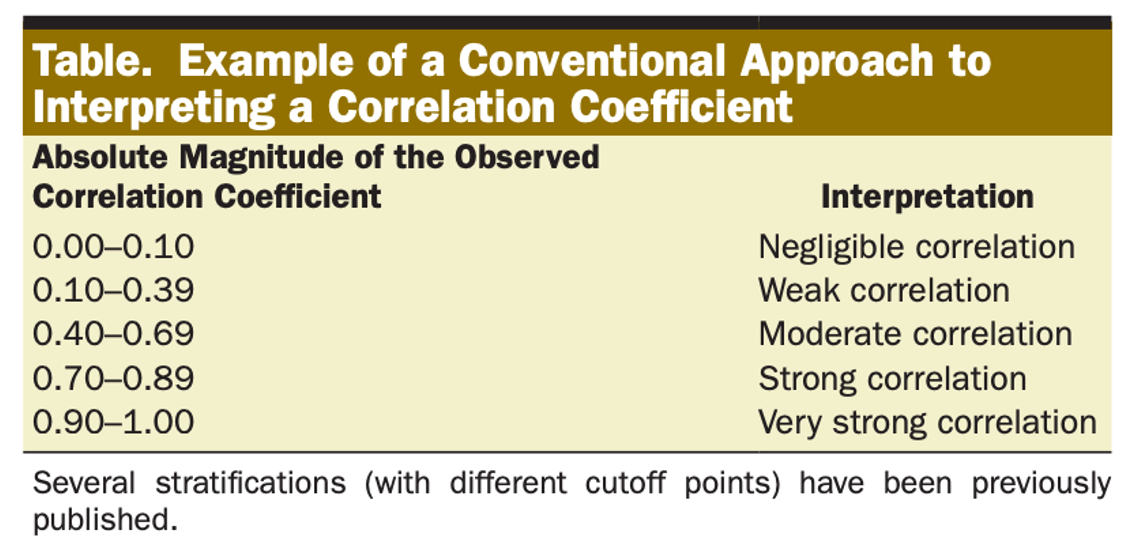
\includegraphics[width=1\linewidth]{img/corr_magn} \caption{Correlatiesterkte}\label{fig:corrmagn}
\end{figure}

\hypertarget{spss}{%
\section*{SPSS}\label{spss}}


In dit hoofdstuk maken we gebruik van de dataset \texttt{tevredenheid}, waarbin \(n=9\) kinesitherapeueten werden bevraagd.

\textbf{Stap 1}: Voer de data in in de \texttt{dataview} van {SPSS}.

\textbf{Stap 2}: Hierna kunnen we de correlaties binnen {SPSS} laten berekenen via \texttt{Analyze\ \textgreater{}\ Correlate\ \textgreater{}\ Bivariate}.

\begin{figure}
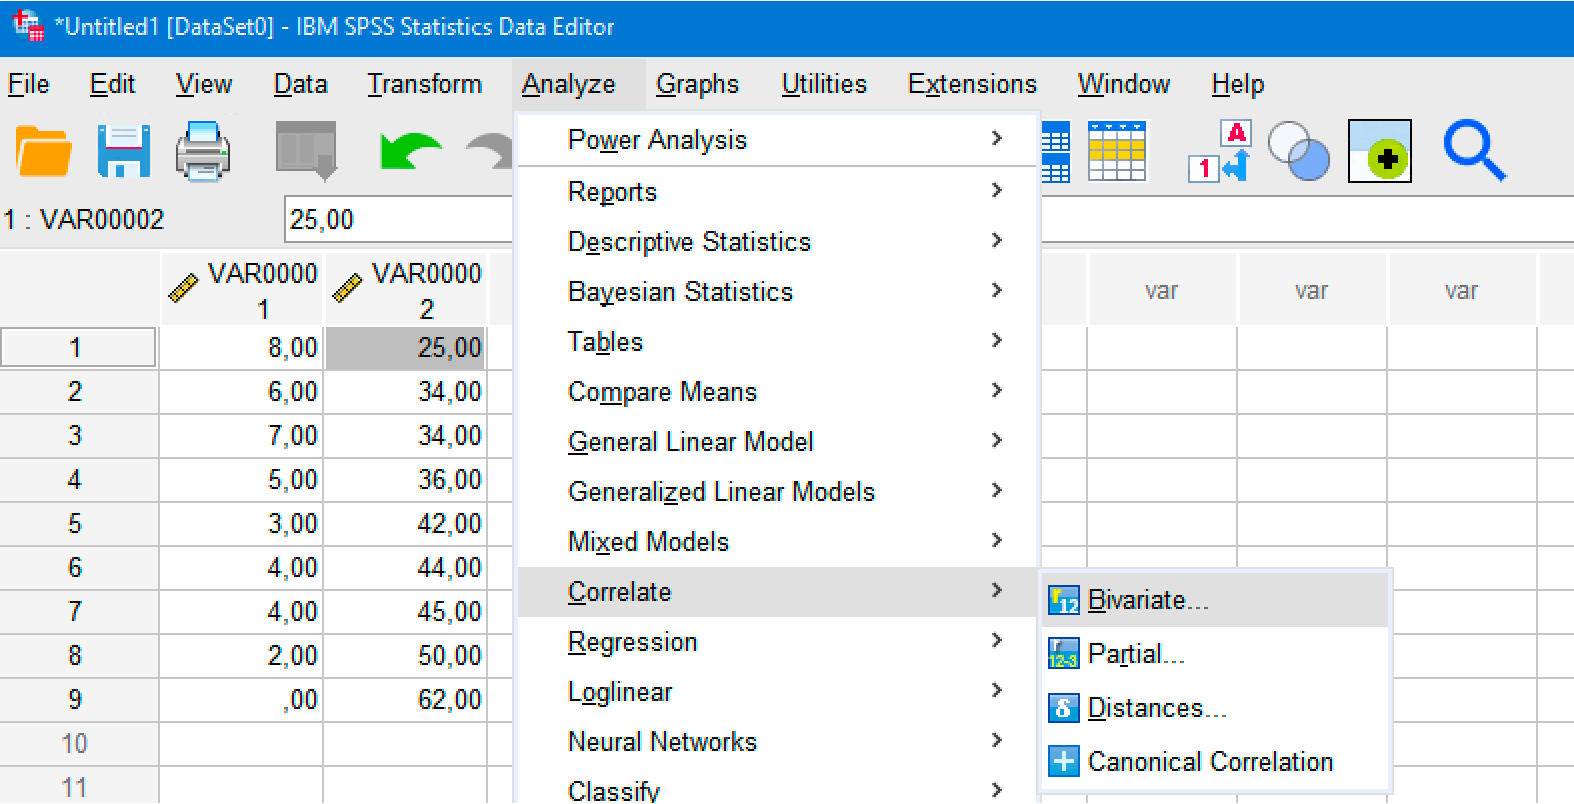
\includegraphics[width=0.75\linewidth]{img/spss_corr_1} \caption{SPSS}\label{fig:corrspss1}
\end{figure}

\textbf{Stap 3}: Hierna krijgen we de pop-up zoals weergegeven in figuur \ref{fig:corrspss2}, waarin we zowel \texttt{Pearson} als \texttt{Spearman} kunnen aanduiden en de verschillend evariabelen waartussen we een correlatie wensen te berekenen. We dienen hierbij minstens 2 variabelen aan de duiden, maar kunnen meerdere variabelen toevoegen. {SPSS} zal automatisch alle 2x2 correlaties berekenen en weergeven in een matrix met op de diagonaal \(\rho = 1\) or \(r_s = 1\).

\begin{figure}
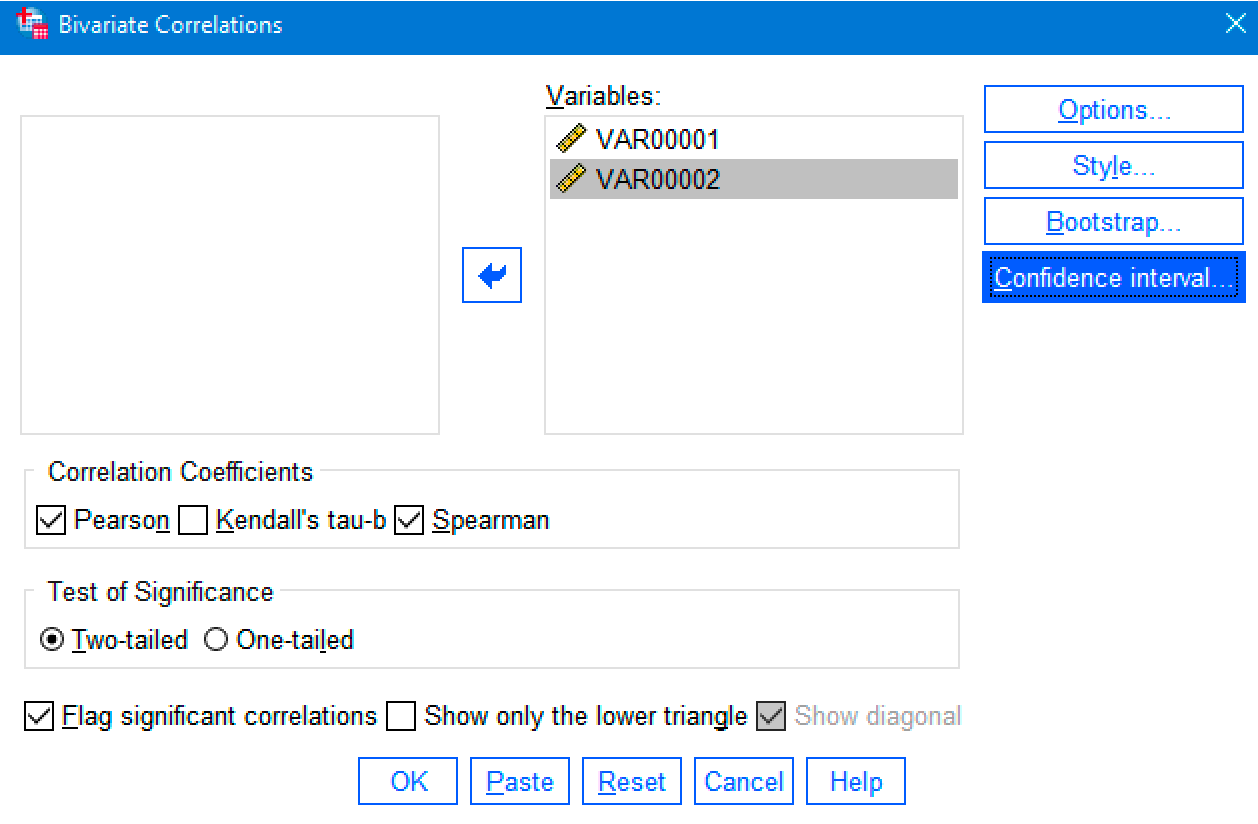
\includegraphics[width=0.75\linewidth]{img/spss_corr_2} \caption{SPSS}\label{fig:corrspss2}
\end{figure}

\textbf{Stap 4}: Vergeet niet om de Syntax te gebruiken binnen {SPSS}.

\begin{figure}
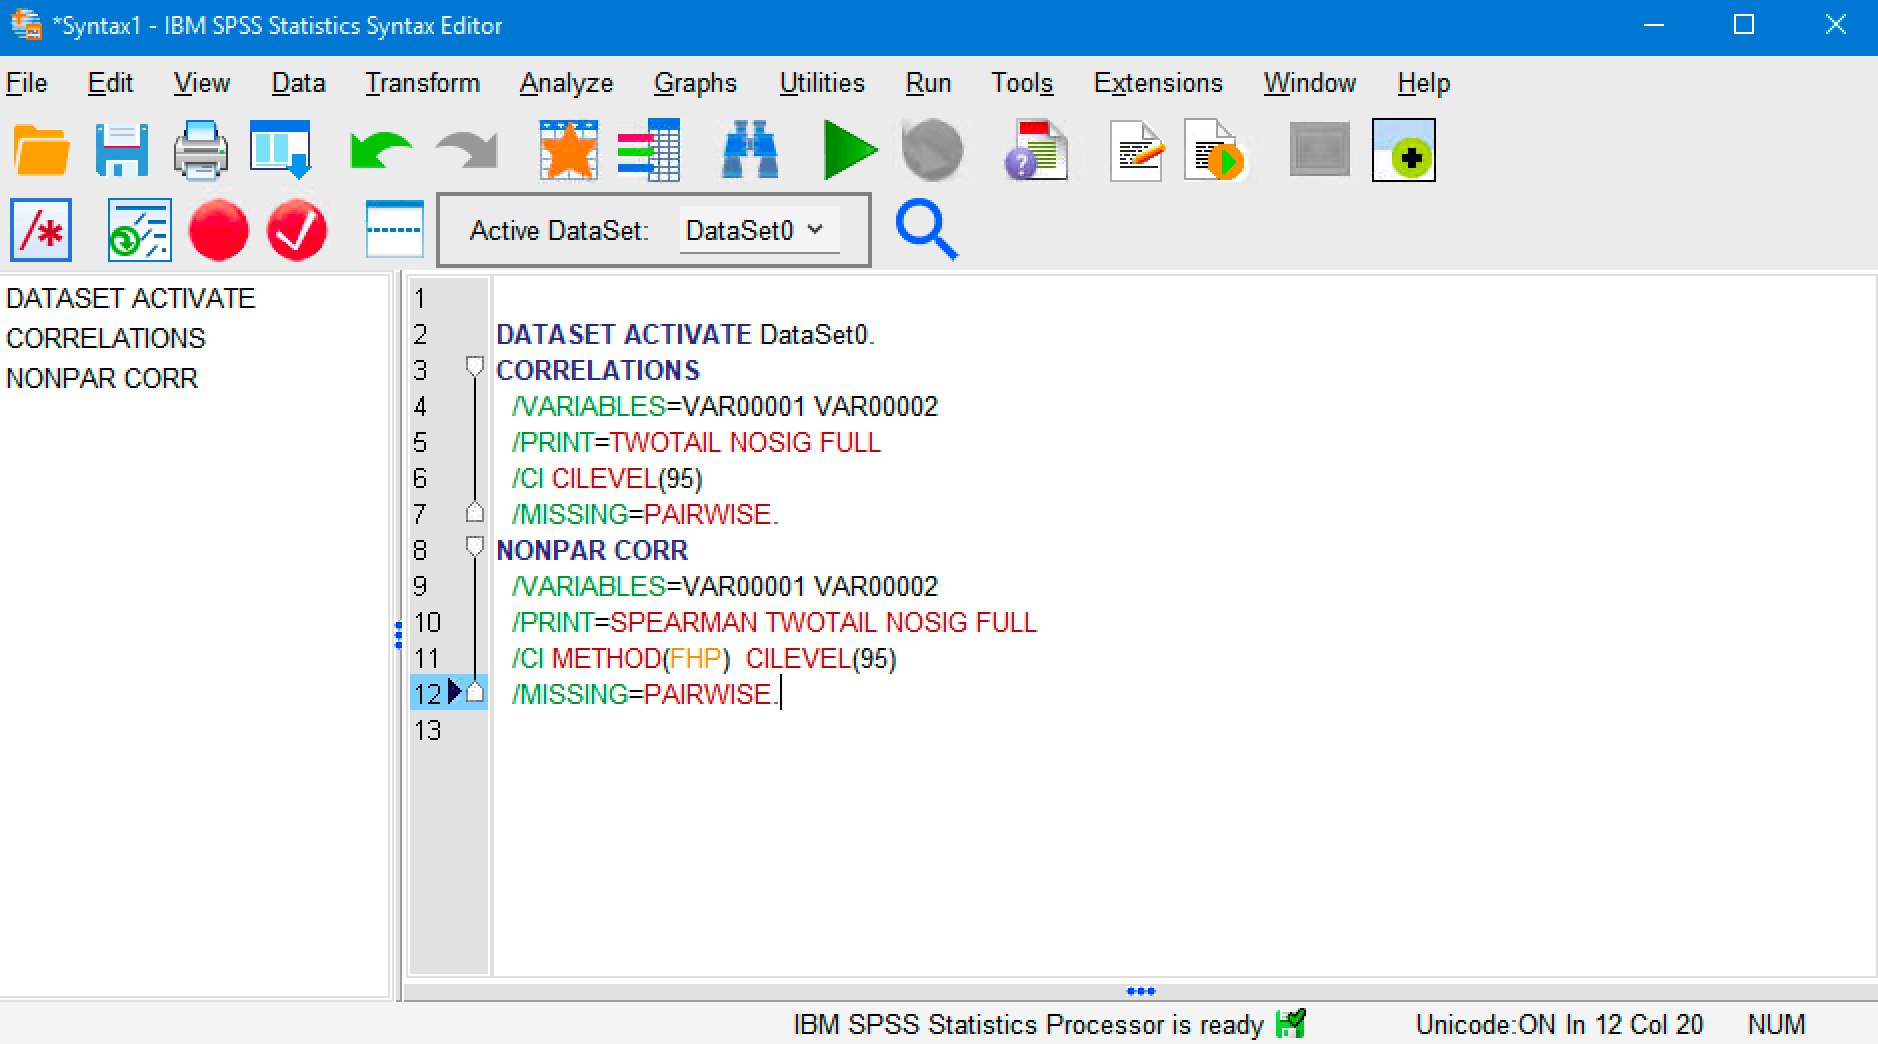
\includegraphics[width=0.75\linewidth]{img/spss_corr_3} \caption{SPSS}\label{fig:corrspss3}
\end{figure}

\textbf{Stap 5}: Tot slot kunnen we de correlaties bekijken en interpreteren. In figuur \ref{fig:corrspss4} vinden we de resultaten voor \(\rho\), terwijl we in figuur \ref{fig:corrspss5} de resultaten voor \(r_s\). We vinden in deze figuren ook de \(p\)-waarde terug en een 95\% betrouwbaarheidsinterval (\(95\% CI\)).

In figuur \ref{fig:corrspss3} zijn de resultaten weergegeven wanneer we de Pearson correlatie berekenen. In figuur \ref{fig:corrspss4} zijn de resultaten weergegeven wanneer we de Spearman correlatie berekenen.

\begin{figure}
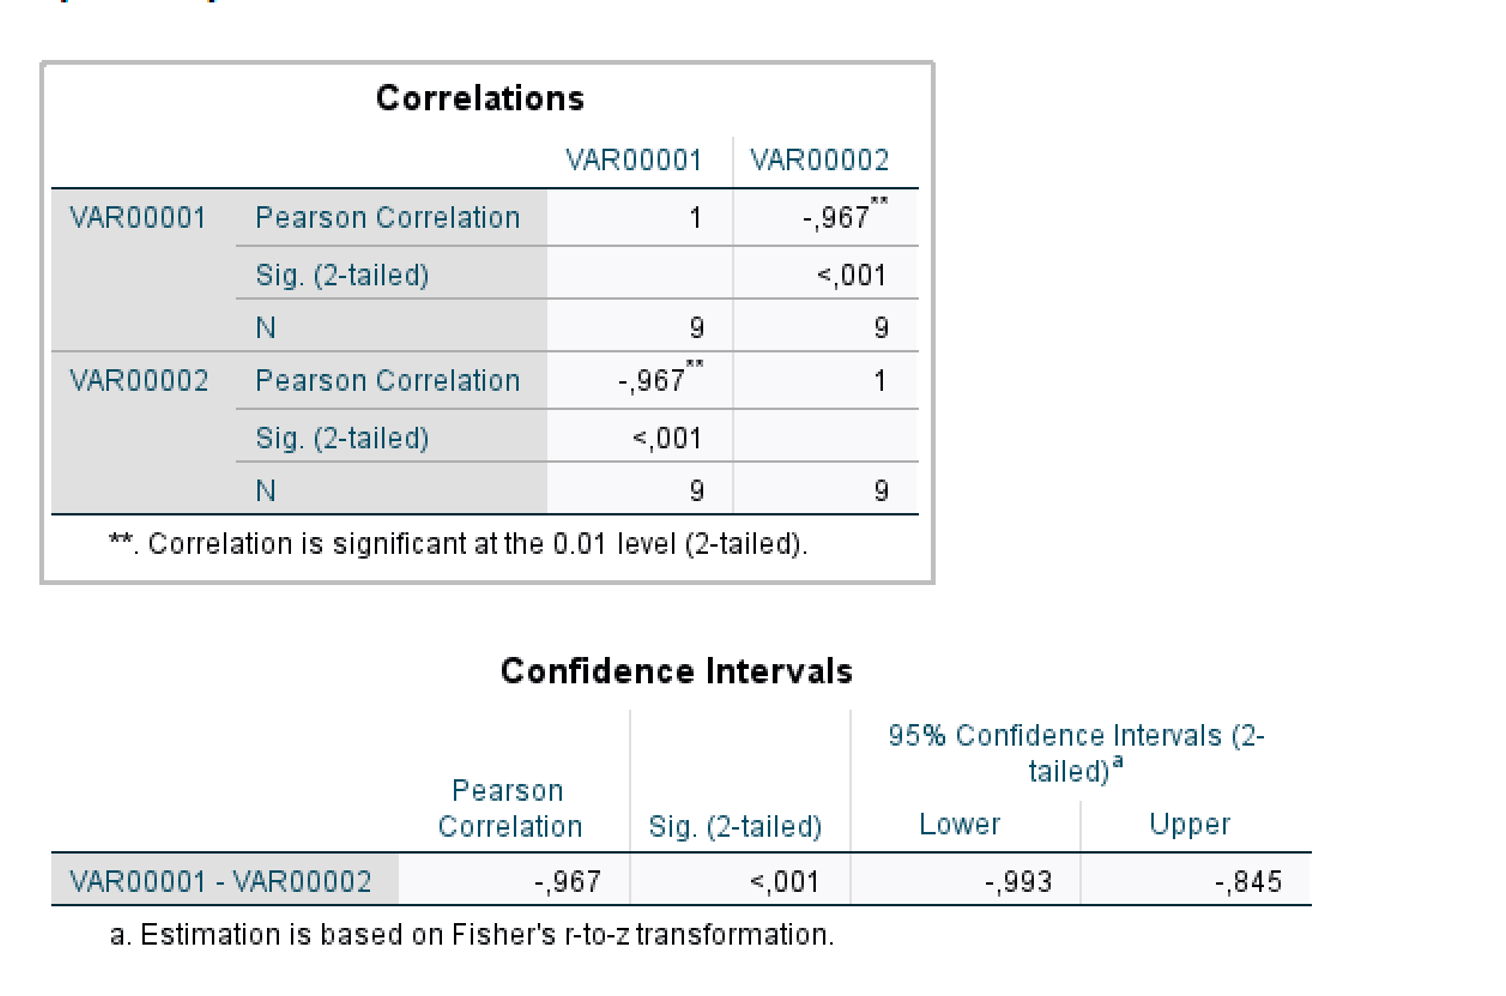
\includegraphics[width=0.75\linewidth]{img/spss_corr_4} \caption{SPSS}\label{fig:corrspss4}
\end{figure}

\begin{figure}
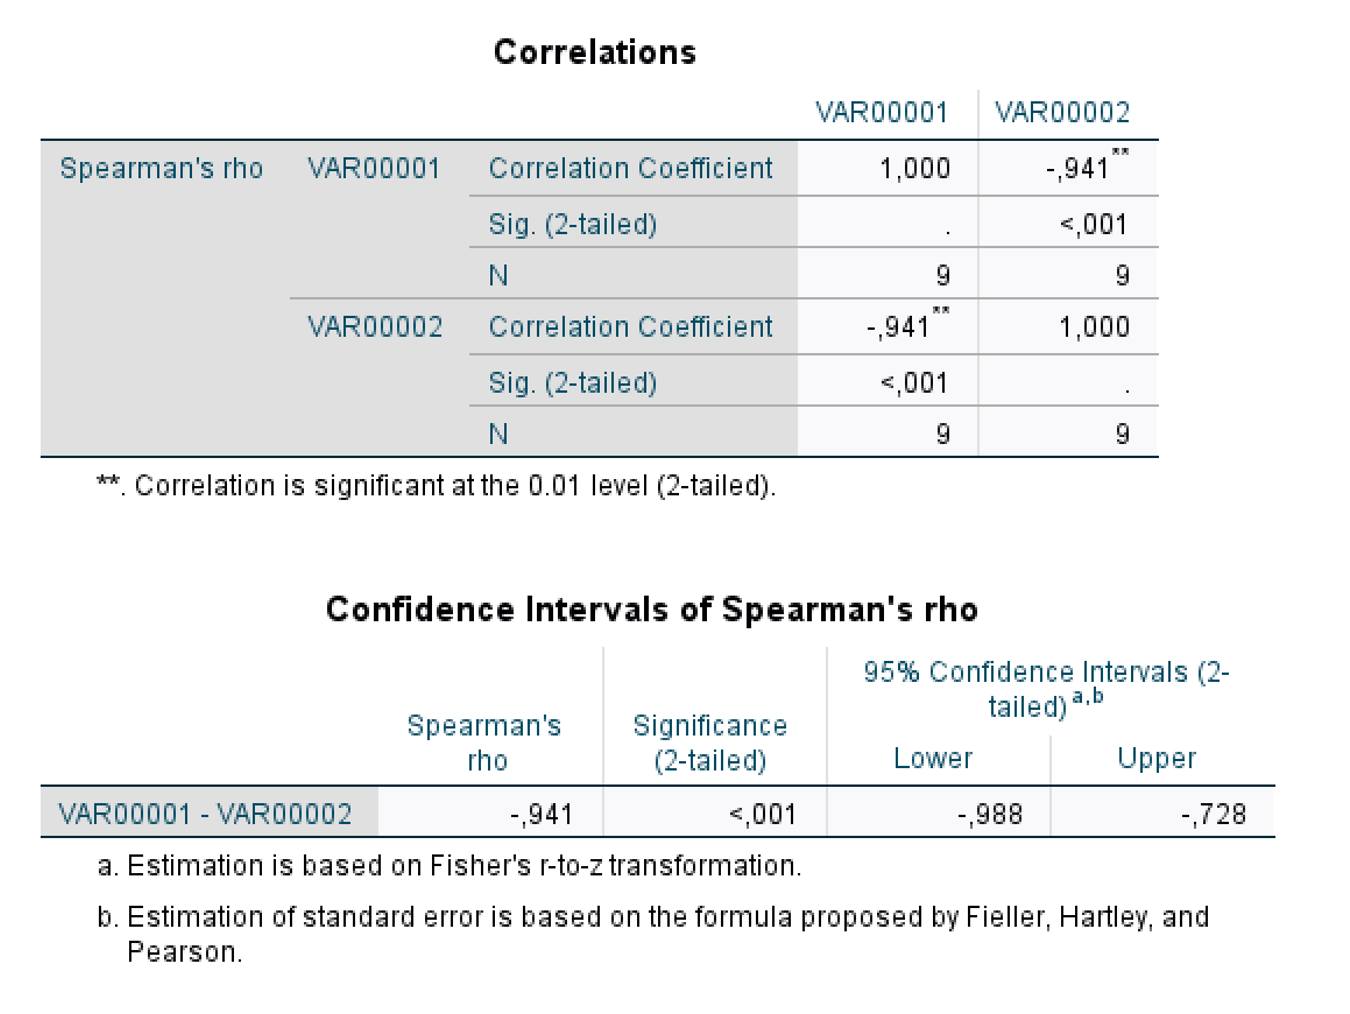
\includegraphics[width=0.75\linewidth]{img/spss_corr_5} \caption{SPSS}\label{fig:corrspss5}
\end{figure}

\newpage

\hypertarget{oefeningen}{%
\section*{Oefeningen}\label{oefeningen}}


In dit onderdeel vinden jullie alle oefeningen over correlaties en associatiaties. De oplossingen worden later gepost op \textbf{Ufora}.

\begin{exercise}

Binnen een onderzoek naar het oplopen van lestel bij sporters, zijn onderzoekers op zoek gegaan naar mogelijke risicofactoren. Ze includeerde 10 sporters, allemaal met een leeftijd van 15 jaar en noteerden de volgende aantal letsels: 5, 0, 0, 2, 2, 3, 1, 2, 1, 0. De onderzoekers waren geïntereseerd in het verband tussen leeftijd en het anatal letsels. Welke van onderstaande stellingen is WAAR:

\begin{itemize}
\tightlist
\item
  Met een correlatie kunnen we niet aantonen wat een risicofactor is en wat niet.
\item
  We kunnen binnen deze studie geen correlatie berekenen.
\item
  Binnen deze studie kunnen we het verband nagaan tussen aantal letsels en leeftijd door een Pearson correlatie te berekenen.
\item
  Binnen deze studie kunnen we het verband nagaan tussen aantal letsels en leeftijd door een Spearman correlatie te berekenen.
\end{itemize}

\end{exercise}

\begin{exercise}

Een correlatie kunnen we steeds weergeven aan de hand van een lijn.

\begin{itemize}
\tightlist
\item
  Waar
\item
  Onwaar
\end{itemize}

\end{exercise}

\begin{exercise}

Een correlatie kunnen we steeds weergeven aan de hand van een lijn.

\begin{itemize}
\tightlist
\item
  Waar
\item
  Onwaar
\end{itemize}

\end{exercise}

Alle volgende oefeningen hebben te maken met volgende klinische studie: \textgreater In een cross-sectionele studie wordt er onderzoek gedaan naar het verband tussen valrisico bij ouderen en de Timed Up and Go (TUG) test. In het totaal zijn er 15 deelnemers binnen de studie waarbij de TUG test wordt afgenomen en de tijd (in s) wordt opgenomen. Verder wordt er bij elke deelnemer ook bevraagd hoevaak ze gevallen zijn het afgelopen jaar.

In onderstaande tabel \ref{tab:TUG} vinden jullie de resultaten van deze studie. Voer deze gegevens ook in binnen de DATA omgeving van {SPSS} en gebruik het programma waar nodig.

\begin{table}

\caption{\label{tab:TUG}Steekproef naar TUG bij opuderen.}
\centering
\begin{tabular}[t]{rr}
\toprule
vallen & TUG (s)\\
\midrule
0 & 9.69\\
4 & 17.38\\
2 & 13.87\\
3 & 15.40\\
6 & 21.25\\
\addlinespace
1 & 6.69\\
8 & 22.65\\
1 & 13.79\\
1 & 11.53\\
0 & 14.32\\
\addlinespace
0 & 7.29\\
1 & 10.82\\
1 & 11.95\\
0 & 13.77\\
4 & 20.01\\
\bottomrule
\end{tabular}
\end{table}

\begin{exercise}

Binnen deze studie zullen we kunnen aantonen dat de tijd voor het uitvoeren van de TUG al dan niet een oorzaak is voor meer/minder vallen binnen de oudere populatie.

\begin{itemize}
\tightlist
\item
  Waar
\item
  Onwaar
\end{itemize}

\end{exercise}

\begin{exercise}
Welke grafiek past het best voor een visualizatie van deze gegevens?
\end{exercise}

\begin{exercise}
Welke correlatie zouden jullie selecteren voor het berekenen van een correlatie en waarom?
\end{exercise}

\begin{exercise}
Geef de schatting weer van de door jou geselecteerde correlatiecoëfficiënt tot 2 cijfers na de komma en geef een correcte interpretatie aan deze correlatie.
\end{exercise}

\hypertarget{conclusies}{%
\section*{Conclusies}\label{conclusies}}


\begin{itemize}
\tightlist
\item
  Correlatie \(\neq\) een causaal verband.
\item
  Een correlatie kan gebruikt worden om de sterkte van een lineair \(\rho\) of monotoon \(r_s\) verband uit te drukken.
\item
  De \(p\)-waarde van een correlatie zegt niets over de sterkte van de correlatie.
\end{itemize}

\mainmatter

\hypertarget{regr}{%
\chapter{Lineare regressie}\label{regr}}

In de paper van Chester et al.~(2016) vermeld men volgende stelling:

\begin{quote}
``At 6 weeks only, a better outcome for both measures was associated with no previous compared to a previous major operation (shoulder surgery excluded) (SPADI, \(\beta\) = -3.66 to -12.56).''

---Chester et al.~(2016)
\end{quote}

\begin{itemize}
\tightlist
\item
  Kunnen we hieruit besluiten dat er een statistisch significant verschil is in uitkomst na kinesitherapie tussen patiënten met een vroegere operatie vs geen operatie?
\end{itemize}

In dezelfde studie lezen we:

\begin{quote}
``There was no significant difference in mean age or sex between consenters (57 years, SD = 15, 44\% male) and non-consenters (56 years, SD = 16, 47\% male).''

---Chester et al.~(2016)
\end{quote}

\begin{itemize}
\tightlist
\item
  Kunnen we hieruit besluiten dat er geen baseline verschil is tussen mensen die deelnamen aan de volledige studie vs mensen die vroegtijdig de studie hebben verlaten?
\end{itemize}

\hypertarget{inleiding-1}{%
\section*{Inleiding}\label{inleiding-1}}


Lineaire regressie kan zowel toegepast worden in een cross-sectioneel design als prospectieve cohorte en wordt vaak gebruikt voor volgende doelstellingen:

\begin{itemize}
\tightlist
\item
  Het voorspellen van een uitkomstmaat op basis van één of meerdere factoren.
\item
  Het beschrijven van een verband tussen de uitkomstmaat en andere factoren, waarbij rekening wordt gehouden met verstorende variabelen.
\end{itemize}

In essentie is een lineair regressie model opgebouwd uit twee componenten:

\begin{itemize}
\tightlist
\item
  De afhankelijke uitkomstvariabele (\(Y\)), welke een continue variabele dient te zijn.
\item
  De onafhankelijke variabele(n) (\(X\)), welke zowel continu als categorisch van aard kunnen zijn.
\end{itemize}

\(Y = \beta_0 + \beta_1 X_1\)

Wanneer er slechts één onafhankelijke variabele \(X_1\) spreken we van een enkelvoudig lineair regressiemodel. Indien er meerdere onafhankelijke variabelen \(X_1, X_2, X_3,..., X_i\) spreken we van een meervoudig lineair regressiemodel.

\textbf{Een regressiemodel} bestaat uit twee delen, een afhankelijk deel (de uitkomst of wat er geschat moet worden) en een onafhankelijk deel (de verklarende variabelen).

\hypertarget{studie-naar-tevredenheid-1}{%
\section*{Studie naar tevredenheid}\label{studie-naar-tevredenheid-1}}


Gegeven is de volgende dataset \texttt{tevreden} met informatie over een bevraging bij kinesitherapeuten over hun tevredenheid van honoraria.

\begin{itemize}
\tightlist
\item
  \(Y\): tevredenheid (schaal 0-10)
\item
  \(X\): leeftijd (jaren)
\item
  \(Z\): geslacht (M/V)
\end{itemize}

We beschikken in deze specifieke steekproef over een totaal van 9 observaties (\(n = 9\)).

de dataset ziet er als volgt uit:

\begin{table}

\caption{\label{tab:tevereden2}Steekproef naar tevredenheid bij kinesitherapeuten.}
\centering
\begin{tabular}[t]{rrl}
\toprule
X & Y & Z\\
\midrule
25 & 8 & M\\
34 & 6 & M\\
34 & 7 & V\\
36 & 5 & V\\
42 & 3 & V\\
\addlinespace
44 & 4 & M\\
45 & 4 & V\\
50 & 2 & V\\
62 & 0 & M\\
\bottomrule
\end{tabular}
\end{table}

Als we de relatie visueel willen weergeven tussen de leeftijd en tevredenheid over de honoraria, kunnen we gebruik maken van een spreidingsdiagram, welk er als volgt uitziet:

\includegraphics{ugent-ebmstatIII_files/figure-latex/unnamed-chunk-7-1.pdf}

Lineaire regressie geeft net als \(\rho\) het lineaire verband weer (in tegenstelling tot \(r_s\), waarbij het monotone verband geschat wordt). Op basis van \(X\) en \(Y\) uit de \texttt{tevreden}dataset werd volgend regressiemodel geschat:

\(Y = 13.6 + (-0.2)X\)

\textbf{Interpretatie}: Wanneer de leeftijd \(X\) toeneemt met één jaar, dan daalt (\(-\)) de tevredenheidscore die gegeven werd door de kinesitherapeuten gemiddeld met 0.2 (\(\beta_1\)). De interpretatie van het getal 13.6 \(\beta_0\) heeft vaak geen reële betekenis. In deze studie geeft de waarde 13.6 weer wat de gemiddelde score zou zijn voor kinesitherapeuten met een leeftijd van 0 jaar.

\includegraphics{ugent-ebmstatIII_files/figure-latex/unnamed-chunk-8-1.pdf}

Op basis van \(Z\) en \(Y\) uit de \texttt{tevreden}dataset werd volgend regressiemodel geschat:

\(Y = 4.5 + (-0.3)Z\)

\textbf{Interpretatie}: Wanneer we de gemiddelde tevredenheid uitrekenen voor mannen en vrouwen bekomen we volgend resultaat zoals weergegeven in tabel \ref{tab:tevredenmean}. Om tot een numerieke oplossing te komen werden de \texttt{labels} gehercodeerd naar \(0\) voor \(V\) en \(1\) voor \(M\). De waarde van \(\beta_1\) bedraagt nu -0.3, wat het gemiddelde verschil weergeeft tussen mannen en vrouwen voor tevredenheidscore. \(\beta_0\) geeft in dit geval de score weer voor \(Z=0\) (score gegveen door vrouwen).

\begin{table}

\caption{\label{tab:tevredenmean}Gemiddelde tevredenheid bij kinesitherapeuten per geslacht.}
\centering
\begin{tabular}[t]{lr}
\toprule
z & y\\
\midrule
M & 4.5\\
V & 4.2\\
\bottomrule
\end{tabular}
\end{table}

\hypertarget{eigenschappen-van-een-lineair-regressiemodel}{%
\section*{Eigenschappen van een lineair regressiemodel}\label{eigenschappen-van-een-lineair-regressiemodel}}


\hypertarget{schatten-van-lineaire-regressie}{%
\subsection*{Schatten van lineaire regressie}\label{schatten-van-lineaire-regressie}}


Eén van de belangrijste evaluatiecriteria bij een lineair regressiemodel is de meerwaarde van \(X\) in het verklaren van \(Y\). Indien we geen informatie zouden hebben over leeftijd en geslacht, kunnen we \(Y\) het best beschrijven aan de hand van het gemiddelde \(\bar{Y}\).

\includegraphics{ugent-ebmstatIII_files/figure-latex/unnamed-chunk-9-1.pdf}

Om de waarde van de \(X\) variabele in te schatten in het verklaren van \(Y\), kijken we naar de afstand tussen de geschatte regressielijn en de observaties (punten op de grafiek). Wanneer de punten dichter tegen de lijn liggen in vergelijking met een schatting op basis van het algemene gemiddelde \(\bar{Y}\), dan lijkt het dat \(X\) een deel van \(Y\) lijkt te verklaren. Wanneer we \(Y\) willen schatten op basis van de regressielijn, dan duiden we deze schatting aan met \(\hat{Y}\). Zo zal voor \(X = 30\), \(\hat{Y} = 13.6 + (-0.2)30 = 7.6\).

Het verklaarde deel wordt uitgedrukt als verklaarde variantie. Het becijferen van deze verklaarde variantie gebeurt aan de hand van ANOVA tabellen. Zoals weergegeven in figuur \ref{fig:lmsst} varieert \(Y\) over verschillende waarden. De blauwe bollen geven de observaties weer, terwijl de blauwe horizontale lijn het gemiddelde van \(Y\) weergeeft. De afstand van een observatie (blauwe bol) tot de horizontale lijn, maakt onderdeel uit van de totale variantie. Deze totale variantie wordt ook wel de kwadratensom (Sum of Squares) genoemd. Wiskundig wordt de totale spreiding gedefinieerd als de Total Sum of Squares (SST) ofwel \(\sum ({Y}_i - \bar{Y})^2\). Deze formule geeft aan dat het de som van alle afstanden betreft tussen de blauwe bollen en de blauwe horizontale lijn. Daarnaast hebben we ook de regressielijn of best passende rechte. De afstand van de blauwe bollen tot deze lijn, noemen we de resterende fout van het model of residu (SSE) wat wiskundig \(\sum ({Y}_i - \hat{Y})^2\) word ofwel het verschiul tussen de blauwe bollen en de regressielijn. Tot slot hebben we de verklaarde variantie van het model, welke uitdruk in welke mate het model meer verklaard van de variantie van \(Y\) t.o.v. \(\bar{Y}\). Dit wordt weergegeven door \(\sum (\hat{Y}_i - \bar{Y})^2\).

\begin{figure}
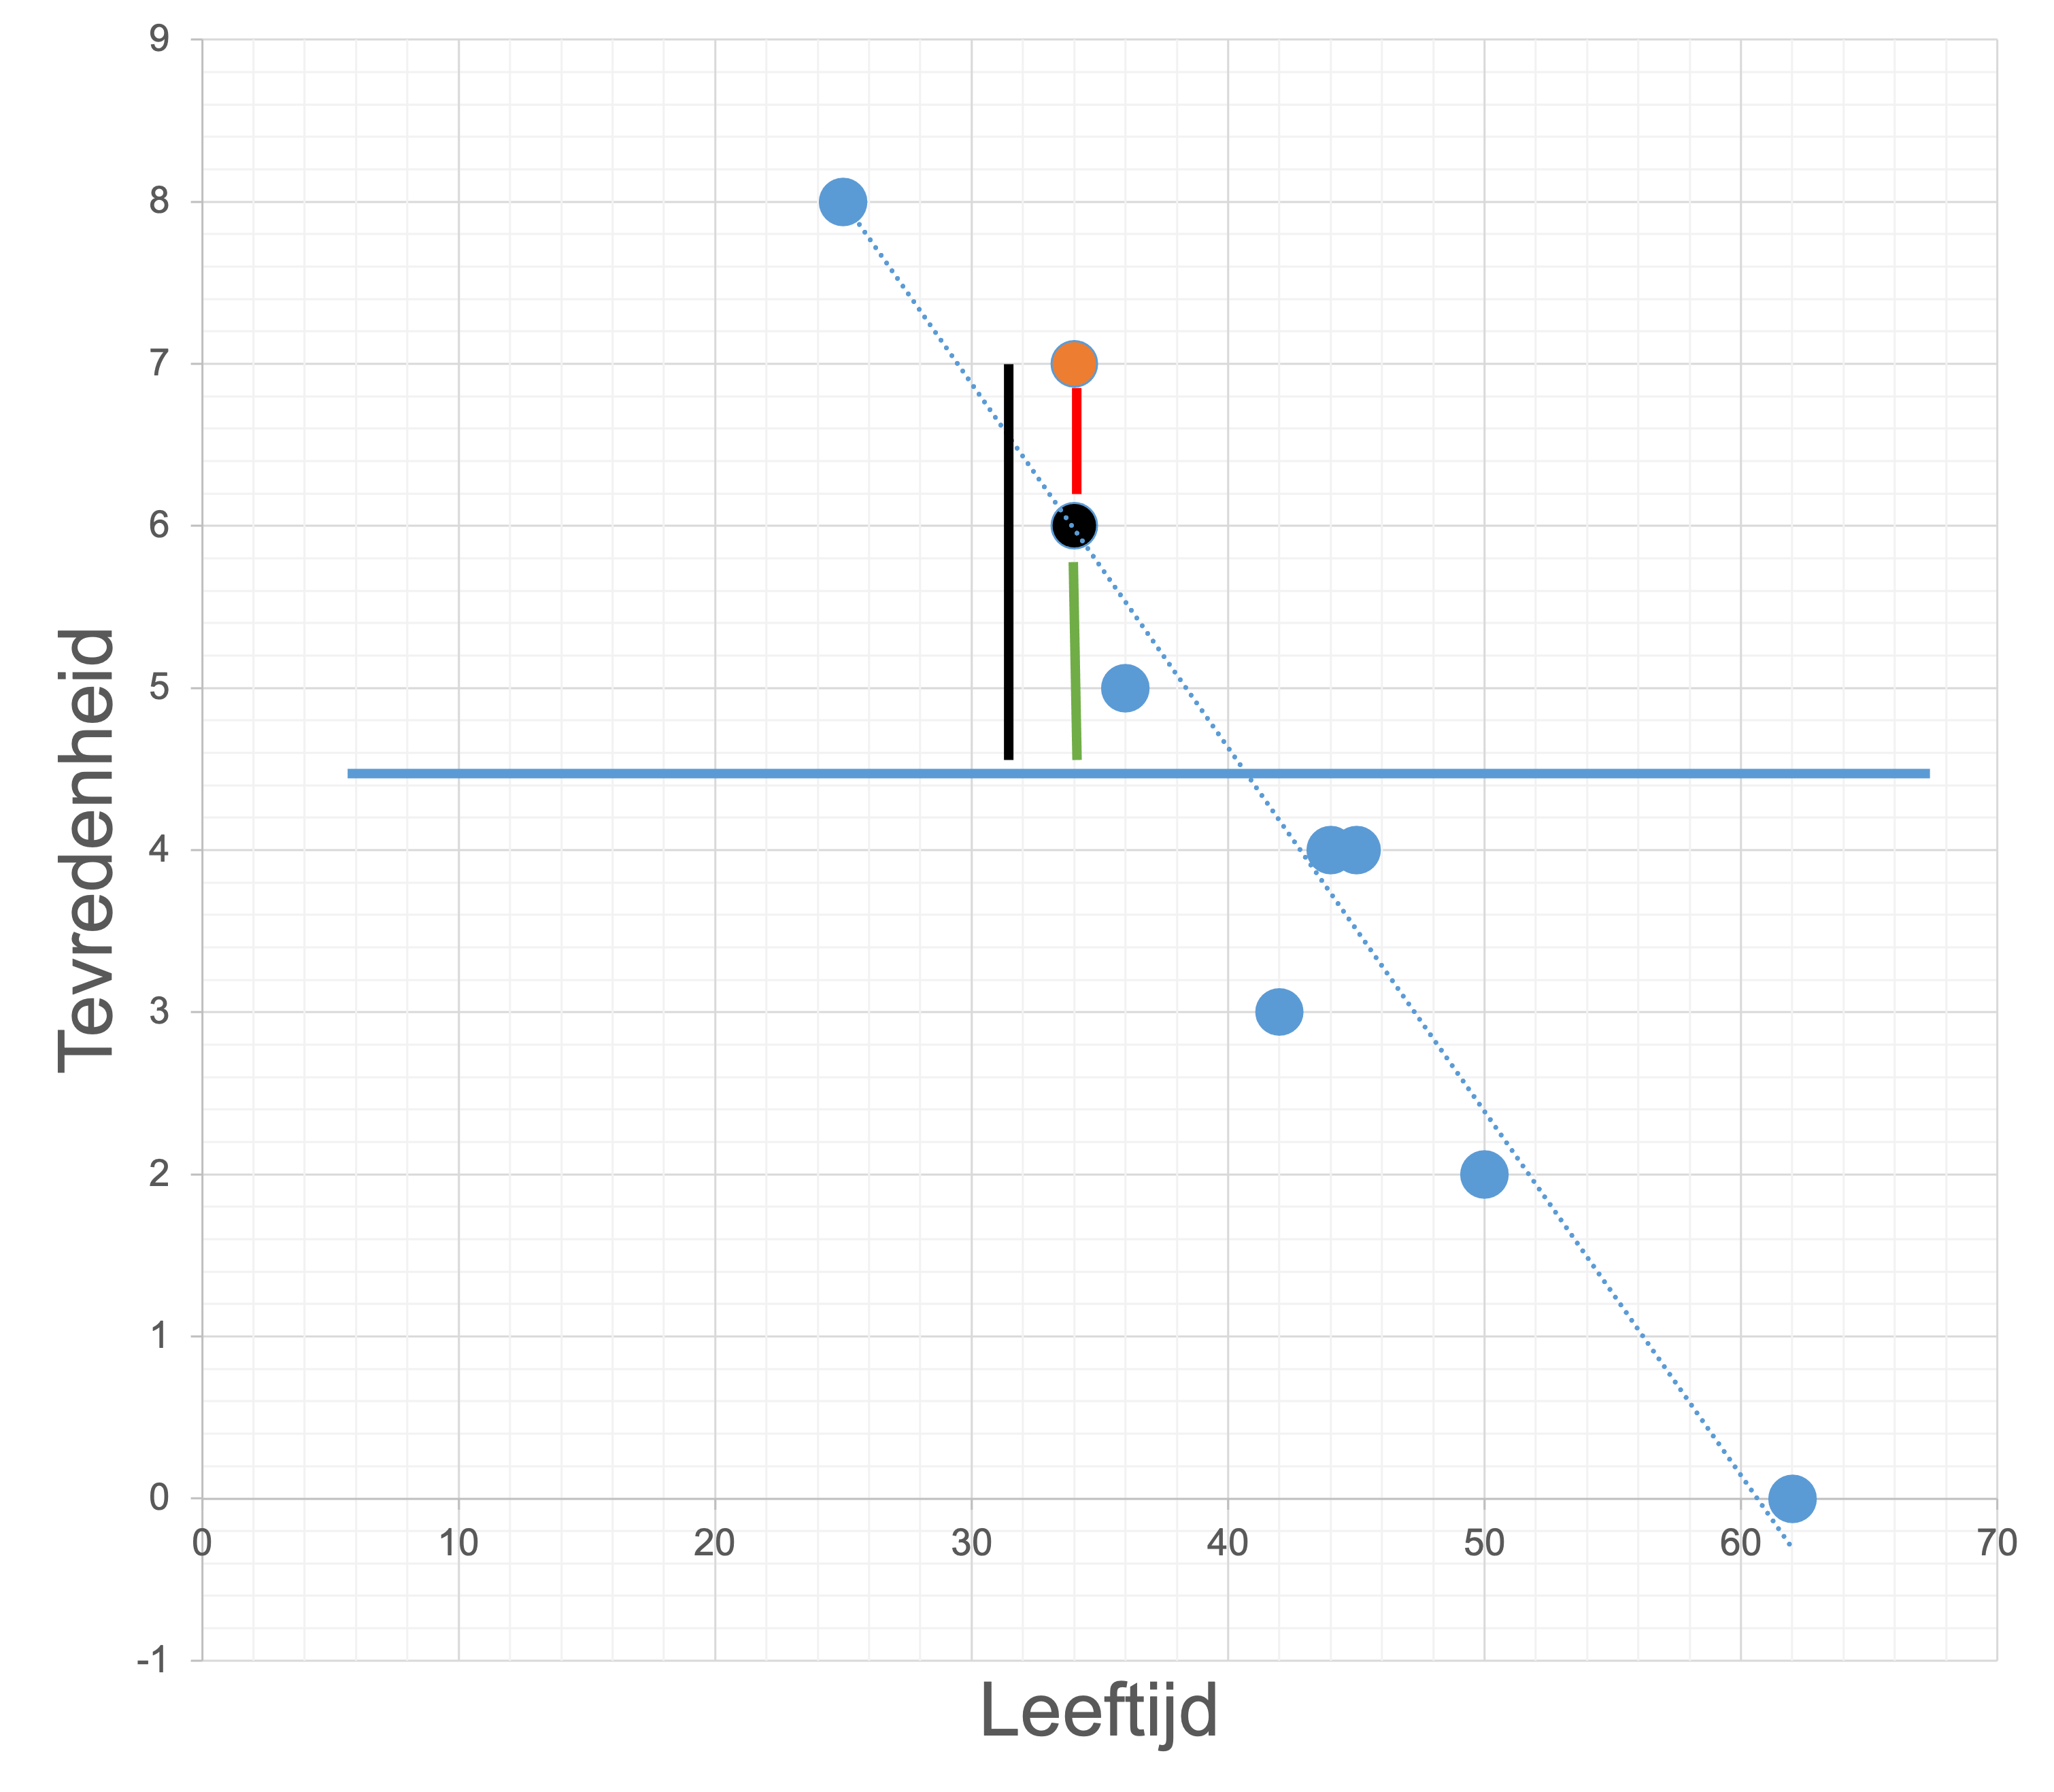
\includegraphics[width=1\linewidth]{img/lm_sst} \caption{Grafische weergave van variantiebronnen}\label{fig:lmsst}
\end{figure}

Uitgewerkt voor de oranje bol (\(X = 34, Y = 7\)) in figuur \ref{fig:lmsst}:

\begin{itemize}
\tightlist
\item
  SST: de afstand tussen de oranje bol \(Y_i\) en de blauwe horizontale lijn \(\bar{Y}\) ofwel \({Y}_i - \bar{Y} = 7 - 4,3 = 2,7\).
\item
  SSE: de afstand tussen de oranje bol \(Y_i\) en de regressielijn \(\hat{Y}\) voor \(X = 34\) ofwel \({Y}_i - \hat{Y} = 7 - (13.6 + (-0.2) \times 34) = 7 - 6 = 1\). (\textbf{opmerking}: hier werden alle cijfers na de komma meegenomen, het volledige model is: \(\beta_0 = 13.6177\) en \(\beta_1 = -0.02246\)).
\item
  SSR: de afstand tussen \(\hat{Y}\) en \(\bar{Y}\).
\end{itemize}

Wanneer we deze oefening voor alles observaties zouden herhalen en kwadrateren en optellen, komen we tot de uiteindelijke kwadratensom.

\begin{table}

\caption{\label{tab:unnamed-chunk-10}Opbouw kwadratensom (1)}
\centering
\begin{tabular}[t]{rrr}
\toprule
SST & SSE & SSR\\
\midrule
3.6666667 & -0.0021598 & 3.6688265\\
1.6666667 & 0.0194384 & 1.6472282\\
2.6666667 & 1.0194384 & 1.6472282\\
0.6666667 & -0.5313175 & 1.1979842\\
-1.3333333 & -1.1835853 & -0.1497480\\
\addlinespace
-0.3333333 & 0.2656587 & -0.5989921\\
-0.3333333 & 0.4902808 & -0.8236141\\
-2.3333333 & -0.3866091 & -1.9467243\\
-4.3333333 & 0.3088553 & -4.6421886\\
\bottomrule
\end{tabular}
\end{table}

Wanneer we al deze waarden kwadrateren komen we tot volgende tabel:

\begin{table}

\caption{\label{tab:unnamed-chunk-11}Opbouw kwadratensom}
\centering
\begin{tabular}[t]{rrr}
\toprule
SST & SSE & SSR\\
\midrule
13.4444444 & 0.0000047 & 13.4602878\\
2.7777778 & 0.0003779 & 2.7133608\\
7.1111111 & 1.0392547 & 2.7133608\\
0.4444444 & 0.2822983 & 1.4351661\\
1.7777778 & 1.4008742 & 0.0224245\\
\addlinespace
0.1111111 & 0.0705746 & 0.3587915\\
0.1111111 & 0.2403752 & 0.6783402\\
5.4444444 & 0.1494666 & 3.7897354\\
18.7777778 & 0.0953916 & 21.5499152\\
\bottomrule
\end{tabular}
\end{table}

Tot slot tellen we alles op:

\begin{table}

\caption{\label{tab:unnamed-chunk-12}Opbouw kwadratensom (3)}
\centering
\begin{tabular}[t]{lr}
\toprule
  & x\\
\midrule
SST & 50.000000\\
SSE & 3.278618\\
SSR & 46.721382\\
\bottomrule
\end{tabular}
\end{table}

Zoals jullie kunnen opmerken uit de laatste tabel, geldt voor de variantiebronnen dat \(SST = SSE + SSR\).

\newpage

\hypertarget{performantie-van-het-regressiemodel}{%
\subsection*{Performantie van het regressiemodel}\label{performantie-van-het-regressiemodel}}


De performantie of verklarende kracht van het regressiemodel wordt uitgedrukt aan de hand van de \emph{determinatiecoëfficiënt} (\(R^2\)). Deze geeft weer hoeveel van de variantie in \(Y\) verklaard kan worden aan de hand van één of meerdere onafhankelijke \(X\) variabelen. Meer bepaald is \(R^2 = \frac{SSR}{SST} = 1 - \frac{SSE}{SST}\). In het voorbeeld hierboven gegeven is \(R^2 = 0.93\) ofwel \(93%
\). De determinatiecoëfficiënt varieerd tussen 0 en 1 (\(R^2 \in [0,1]\)) en hoe dichter bij \(1\), hoe meer van de variantie verklaard kan worden.

Deze berekening wijkt af van de slides door afronding. In de slides werd er geen afronding meegenomen, maar in dit boek werd dit wel meegenomen.

Een volledig overzicht van alle variantiebronnen is weergegeven in onderstaande tabel:

\begin{table}

\caption{\label{tab:unnamed-chunk-13}Overzicht van alle variantiebronnen}
\centering
\begin{tabular}[t]{llll}
\toprule
Bron & Kwadratensom (SS) & Vrijheidsgraden (df) & Kwadratengemiddelde (MS)\\
\midrule
Regressie & \$\textbackslash{}sum ( \textbackslash{}hat\{Y\}\_i - \textbackslash{}bar\{Y\})\textasciicircum{}2\$ & \$m\$ & \$\textbackslash{}frac\{\textbackslash{}sum ( \textbackslash{}hat\{Y\}\_i - \textbackslash{}bar\{Y\})\textasciicircum{}2\}\{m\}\$\\
Residu/Fout & \$\textbackslash{}sum ( Y\_i - \textbackslash{}hat\{Y\})\textasciicircum{}2\$ & \$n-m-1\$ & \$\textbackslash{}frac\{\textbackslash{}sum ( Y\_i - \textbackslash{}hat\{Y\})\textasciicircum{}2\}\{n-m-1\}\$\\
Totaal & \$\textbackslash{}sum ( Y\_i - \textbackslash{}bar\{Y\})\textasciicircum{}2\$ & \$n-1\$ & \$\textbackslash{}frac\{\textbackslash{}sum ( Y\_i - \textbackslash{}bar\{Y\})\textasciicircum{}2\}\{n-1\}\$\\
\bottomrule
\end{tabular}
\end{table}

De uiteindelijke statistische grootheid op basis waarvan de uiteindelijke \(p\)-waarde berekend wordt, is gebaseerd op een afgeleide van de kwadratensom, namelijk het kwadratengemiddelde. Hiervoor wordt elke kwadratensom gedeeld door de bijhorende vrijheidsgraden. Deze vrijheidsgraden zijn \(n-1\) voor de SST (zoals in de formule van variantie uit eerste/tweede Bachelor), \(m\) voor de SSR (waarbij \(m\) het aantal onafhelijke variabelen weergeeft) en \(n-m-1\) voor de SSE. De F-statistiek wordt uiteindelijk berekend als \(F = MS_{regressie}/MS_{residu}\). Hoe groter de waarde van \(F\), hoe meer de regressie in staat is om variantie te verklaren en hoe sneller een statisch signifcant resultaat gevonden kan worden. Voor het \texttt{tevreden} voorbeeld is \(n-1 = 8\), \(m = 1\) en \(n-m-1 = 8-1-1 = 6\). Hieruit kunnen we \(F\) berekenen als \(F = \frac{46.7}{1}/\frac{3.3}{6} = 84.9\)

\begin{figure}
\includegraphics[width=1\linewidth]{ugent-ebmstatIII_files/figure-latex/Ffig-1} \caption{Grafische weergave van variantiebronnen}\label{fig:Ffig}
\end{figure}

Op basis van de berekende \(F\)-waarde en de nul-distributie zoals weergegeven in figuur \ref{fig:Ffig}, zal de \(p\)-waarde \(< 0.001\). Het regressiemodel is met andere waaorden in staat om een significant deel van de variantie van \(Y\) te verklaren op basis van waarden van \(X\).

Bij uitbreiding naar meervoudige lineaire regressie wordt een model als volgt weergegeven: \(Y = \beta_0 + \beta_1X_1 + \beta_2X_2 + … + \epsilon\), waarbij \(Y\) de afhankelijke continue variabele is, \(X_i\) de onafhenkelijke variabele is, \(\beta_i\) een inschatting is van het verband tussen \(X_i\) en \(Y\) en \(\epsilon\) de fout is die gemaakt wordt door het model (\(Y_i - \hat{Y}_i\)).

\hypertarget{hypothesen}{%
\subsection*{Hypothesen}\label{hypothesen}}


Binnen regressie kunnen er twee hypothesen worden opgesteld: (1) een hypothese over de regressie-analyse zelf en (2) een hypothese over de \(\beta\) coëfficiënten. De hypothese kunnen we algemeen als volgt opstellen:

\begin{itemize}
\tightlist
\item
  \(H_0\): Er is geen verband (\(\beta_i = 0\)) tussen de leeftijd (\(X_i\)) van de therapeut en de gegeven tevredenheidsscore (\(Y_i\)).
\item
  \(H_1\): Er is een verband (\(\beta_i \neq 0\)) tussen de leeftijd (\(X_i\)) van de therapeut en de gegeven tevredenheidsscore (\(Y_i\)).
\end{itemize}

Een significante \(\beta_i\) wil dus zeggen significant verschillend van 0 en dus een meerwaarde om iets te zeggen over \(Y\). \textbf{Let op}: binnen deze hypothesen kan het ook over meervoudige regressie gaan met verschillende \(\beta\) coefficiënten.

\(H_0\) kan in dit geval \(\beta_1 = \beta_2 = \beta_3 = 0\) zijn.

Er wordt nooit een hypothese gevormd over \(\beta_0\). Kan je zelf bedenken waarom dit het geval is?

\hypertarget{voorwaarden-van-een-lineair-regressiemodel}{%
\section*{Voorwaarden van een lineair regressiemodel}\label{voorwaarden-van-een-lineair-regressiemodel}}


Er zijn drie belangrijke voorwaarden vooraleer we regressie-analyse kunnen toepassen:

\begin{itemize}
\tightlist
\item
  Lineariteit
\item
  Onafhakelijke waarnemingen
\item
  Residuen normaal verdeeld met gemiddelde 0 en constante variantie
\end{itemize}

De eerste voorwaarde, \textbf{lineariteit}, houdt in dat een regressieanalyse enkel in staat is om een correcte inschatting te maken van een verband tussen één continue afhankelijke variabele en één of meerdere afhankelijke variabelen als dit verband lineair is. Wanneer het verband niet lineair is, zal de inschatting op basis van lineaire regressie een foutief beeld geven, m.a.w. de schattingen zullen niet valide zijn en er zal \emph{bias} optreden.

De tweede voorwaarde, \textbf{onafhakelijke waarnemingen}, geeft aan dat de klassieke lineaire regressie een inschatting kan maken wanneer er slechts één observatie is per variabele per persoon. Indien eenzelfde variabele meerdere malen gemeten of bevraagd werd bij eenzelfde persoon zal de inschatting van de regressie niet correct zijn. De schatting zal nu niet per se onderhevig zijn aan bias, maar de berekeningen van het \(95\% CI\) zal niet correct kunnen gebeuren.

De derde voorwaarde, \textbf{normaal verdeelde residuen}, geeft aan dat de fouten die door het model gemaakt zijn normaal verdeeld moeten zijn met een gemiddelde van 0. Dit is belangrijk aangezien de regressielijn een gemiddelde weergeeft van \(Y\) (\(\bar{Y}\)) voor elke \(X_i\). Indien de residuen niet normaal verdeeld zijn en het gemiddelde van de residuen niet gelijk zou zijn aan 0, gaat de veronderstelling van een gemiddelde inschatting niet meer op.

\hypertarget{selectie-van-een-regressiemodel}{%
\section*{Selectie van een regressiemodel}\label{selectie-van-een-regressiemodel}}


Er bestaan verschillende automatische selectiemethoden om een regressiemodel te definiëren:

\begin{itemize}
\tightlist
\item
  Forward
\item
  Backward
\item
  Enter
\item
  Stepwise
\end{itemize}

In deze cursus gaan we hier niet verder op in.

\hypertarget{dummy-coding}{%
\section*{Dummy coding}\label{dummy-coding}}


Wanneer we gebruik maken van een onafhankelijke categorische \(X\) variabele die bestaat uit \(>2\) cetagoriën, moeten we dummy coding uitvoeren, aangezien we een variabele met bijvoorbeeld 5 categoriën niet kunnen weergeven aan de hand van één \(\beta\) coëfficiënt. Neem bijvoorbeeld tabel \ref{tab:dummy1}, waarbij we de variabele \texttt{Rookstatus} met drie categoriën gaan opdelen in \(m-1\) variabelen, waarbij \(m\) het aantal categoriëen weergeeft. Op basis van rookstatus wensen we in dit voorbeeld een inschatting te maken van het gewicht (in kg).

\textbf{Hier}: \(3-1 = 2\) dummy categoriën.

\begin{table}

\caption{\label{tab:dummy1}Dummy coding}
\centering
\begin{tabular}[t]{lrr}
\toprule
Rookstatus & Actieve roker & Vroegere roker\\
\midrule
Niet roker & 0 & 0\\
Vroegere roker & 0 & 1\\
Actieve roker & 1 & 0\\
\bottomrule
\end{tabular}
\end{table}

Uit tabel \ref{tab:dummy1} kunnen we op basis van slechts twee nieuwe variabelen de drie oorspronkelijke categoriën steeds opnieuw terughalen. Voor elk van deze nieuwe variabelen wordt er in het regressiemodel een \(\beta\) ingeschat. We krijgen hierdoor volgende regressievergelijking:

\(Y = \beta_0 + \beta_1 X_1 + \beta_2 X_2\), waarbij \(X_1\) de associatie is met \texttt{Actieve\ roker} en \(X_2\) de associatie met \texttt{Vroegere\ roker}.

\begin{itemize}
\tightlist
\item
  \(Y = \beta_0 + \beta_1 (actieve \space roker) + \beta_2 (vroegere \space roker)\)
\item
  \(Y = 64 - 2 \times (actieve \space roker) + 0.5 \times (vroegere \space roker)\)
\end{itemize}

Voor een actieve roker komen we dan volgende schatting uit: \(\hat{Y} = 64 - 2 \times (actieve \space roker = 1) + 0.5 \times (vroegere \space roker = 0)\) ofwel \(\hat{Y} = 64 - 2 \times 1 = 62 \space kg\). Voor elk label binnen de variabele \texttt{Rookstatus}, kunnen we dus de inschatting van het gewicht gaan berekenen.

\begin{exercise}
Kan je zelf voor de andere categoriën deze inschatting maken? Hoe bepaal je het gewicht voor de categorie die is weggevallen?
\end{exercise}

Ook in wetenschappelijke artikels zal je binnen categorische variabelen merken dat er aan dummy coding werd gedaan. Hierbij wordt de referentiecategorie vaak gedefinieerd als \(0\).

\begin{figure}
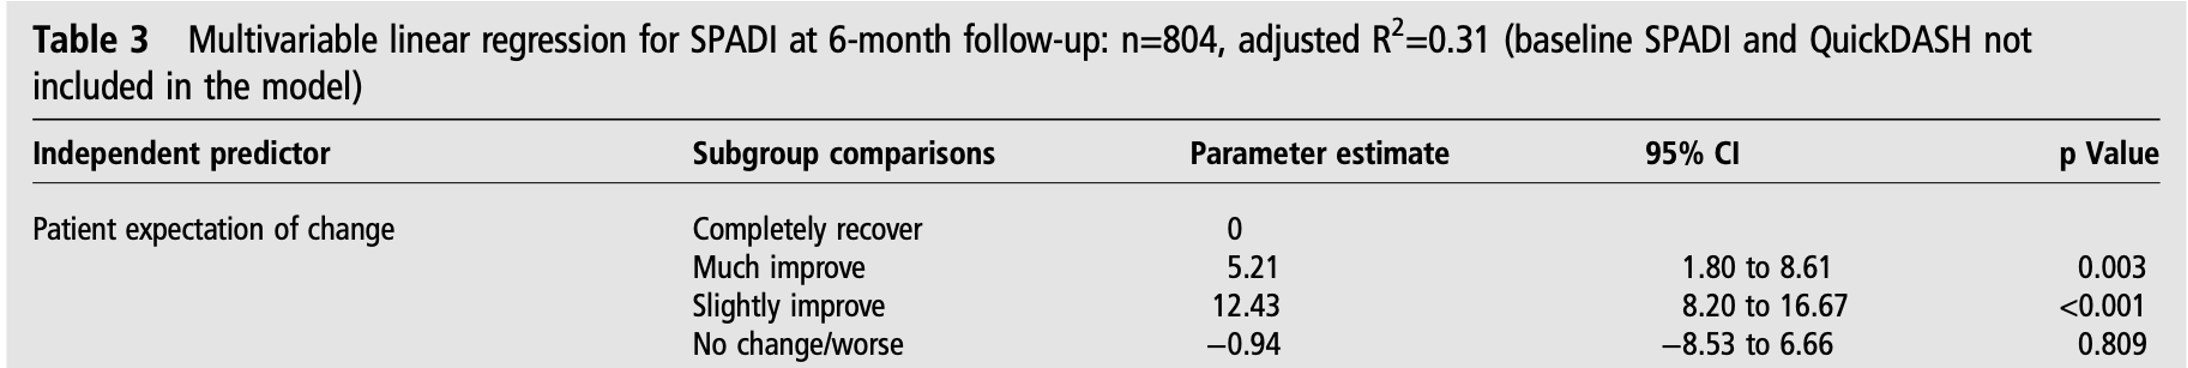
\includegraphics[width=1\linewidth]{img/chester_dummy} \caption{Dummy coding in wetenschappelijk artikel}\label{fig:chesterdummy}
\end{figure}

\hypertarget{multicollineariteit}{%
\section*{Multicollineariteit}\label{multicollineariteit}}


Wanneer we gebruiken maken van meervoudige lineaire regressie, kan er multicollienariteit optreden. Hierbij zijn de verschillende onafhankelijke variabelen onderling gecorreleerd. Multicollienariteit heeft invloed op schatten van de regressiecoëffi¨cnten, betrouwbaarheidsintervallen, etc\ldots{}

Binnen {SPSS} kunnen we hiervoor \texttt{Collinearity\ diagnostics} aanduiden. De twee meest gebruikte schattingen voor collineariteit zijn:

\begin{itemize}
\tightlist
\item
  Tolerance (waarde dicht bij 0 wijst op multicoll.) = \% variantie in de onafh. dat niet kan worden verklaard door de andere onafh. variabelen
\item
  Variance Inflation Factor (VIF) = reciproke waarde van de `Tolerance' (hoge waarde wijst op multicoll.)
\end{itemize}

\hypertarget{spss-en-oefeningen}{%
\section*{SPSS en oefeningen}\label{spss-en-oefeningen}}


In dit deel kunnen jullie voor het eerst kennis maken met lineaire regressie binnen het statistisch softwareprogramma SPSS. Probeer op een gestructureerde manier alle stappen in dit document te volgen en hierna ook de vragen te beantwoorden.

Als kinesitherapeut binnen een obesitaskliniek wil je het verband tussen het BMI (kg/m²) van de patiënten en de uitkomst van de 6-minuten wandeltest (6MWT) in kaart brengen. Gegeven is de volgende dataset:

\begin{table}

\caption{\label{tab:unnamed-chunk-14}Overzicht van data binnen obesitaskliniek}
\centering
\begin{tabular}[t]{rr}
\toprule
BMI (kg/m2) & 6MWT (meter)\\
\midrule
23 & 120\\
28 & 108\\
26 & 105\\
22 & 115\\
31 & 95\\
\addlinespace
26 & 95\\
32 & 82\\
36 & 87\\
42 & 40\\
\bottomrule
\end{tabular}
\end{table}

\begin{exercise}
Bereken de SST voor uitkomst van de 6MWT. Vergeet niet dat de SST berekend wordt door enkel rekening te houden met het gemiddelde.
\end{exercise}

\begin{exercise}
Het verband tussen de 6MWT en het BMI wordt weergegeven aan de hand van volgende formule: \(Y = 195.5 – 3.4X\) OF: \(6MWT = 195.5 – 3.4 \times BMI\) Kan je voorspellen wat de uitkomst op de 6MWT zou zijn voor een person met een BMI van 30?
\end{exercise}

\begin{exercise}
Bereken nu de SSE voor de uitkomst van de 6MWT op basis van bovenstaand regressie-model. Kan je ook de determinatiecoëfficiënt (\(R^2\)) berekenen?
\end{exercise}

Open SPSS en voeg de data in die in de les gebruikt werd voor het beschrijven van het verband tussen de tevredenheid van kinesitherapeuten over hun honoraria en hun leeftijd. Uiteindelijk zou je volgende dataset moeten hebben ingegeven:

\begin{figure}
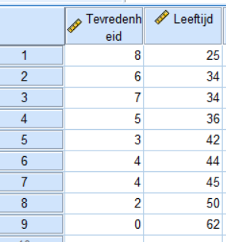
\includegraphics[width=1\linewidth]{img/ex_spss_lm_1} \caption{Data voor tevredenheid}\label{fig:exspsslm1}
\end{figure}

Ga naar \texttt{analyze\ \textgreater{}\ regression\ \ \textgreater{}\ linear} en vul daar volgende gegevens aan:

\begin{figure}
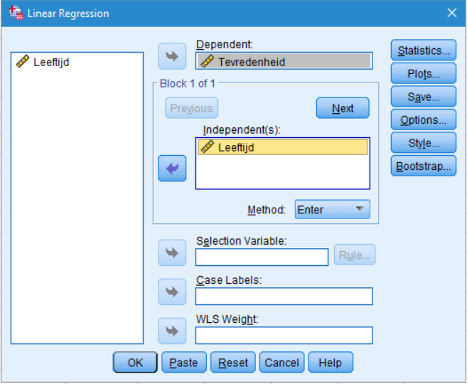
\includegraphics[width=1\linewidth]{img/ex_spss_lm_2} \caption{Model invullen}\label{fig:exspsslm2}
\end{figure}

Let er op dat we tevredenheid onder dependent (afhankelijk) plaatsen en leeftijd onder independent (onafhankelijke). Klik hierna op \texttt{Statistics...} en selecteer onder de statistieken ``confidence intervals''. Klik hierna op \texttt{Paste} en voer de Syntax uit.

\begin{exercise}
Kan je in de output het regressiemodel terugvinden?
\end{exercise}

\begin{exercise}
Is er een significant verband tussen de leeftijd en de score voor tevredenheid? Waaruit leid je dit af?
\end{exercise}

\begin{exercise}
Waarvoor staat het 95\% CI? Kan je dit interpreteren?
\end{exercise}

Open SPSS en voeg de data in die in de les gebruikt werd in oefening 1. Uiteindelijk zou je volgende dataset moeten hebben ingegeven:

\begin{figure}
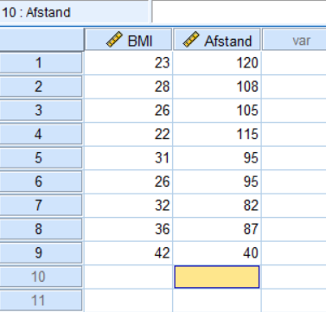
\includegraphics[width=1\linewidth]{img/ex_spss_lm_3} \caption{Data voor obesitas}\label{fig:exspsslm3}
\end{figure}

Ga naar \texttt{analyze\ \textgreater{}\ regression\ \ \textgreater{}\ linear} en vul daar volgende gegevens aan:

\begin{figure}
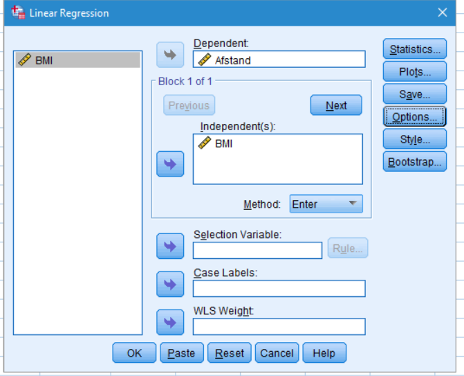
\includegraphics[width=1\linewidth]{img/ex_spss_lm_4} \caption{Model invullen obesaitas}\label{fig:exspsslm4}
\end{figure}

Klik hierna op \texttt{Statistics...} en selecteer onder de statistieken ``confidence intervals''. Klik hierna op \texttt{Paste} en voer de Syntax uit.

\begin{exercise}
Kan je in de output de fouten terugvinden die het model maakt (SSE en SST)? Wat is de waarde van de SSE?
\end{exercise}

\begin{exercise}
Is er een significant verband tussen de BMI en de 6MWT? Wat is de p-waarde voor deze associatie?
\end{exercise}

\begin{exercise}
Waarvoor staat het 95\% CI? Kan je dit interpreteren?
\end{exercise}

Probeer ook nog even volgende meerkeuzevragen te beantwoorden:

\begin{exercise}

Ik heb een categorische variabele over het opleidingsniveau welke bestaat uit 5 mogelijke antwoorden. Selecteer het correcte antwoord.

\begin{itemize}
\tightlist
\item
  Ik kan deze variabele zo toevoegen in het lineaire model in SPSS.
\item
  Ik zal deze moeten hercoderen naar 5 nieuwe variabelen.
\item
  Ik zal deze moeten hercoderen naar 4 nieuwe variabelen.
\item
  Ik zal deze moete hercoderen naar een continue variabele met schaal 1 t.e.m. 5.
\end{itemize}

\end{exercise}

\begin{exercise}

Als ik een lineair model maak in SPSS, dan\ldots{}

\begin{itemize}
\tightlist
\item
  Is het belangrijk dat ik steeds de lineariteit, multicollineariteit en normaalverdeling van de residuen bekijk.
\item
  Dien ik eerst te kijken naar de VIF om multicollineariteit na te gaan.
\item
  Dien ik gebruik te maken van een spearman correlatiecoeffiënt om lineariteit na te gaan.
\end{itemize}

\end{exercise}

\begin{exercise}

Wanneer je verschillende onafhankelijke variabelen hebt, is het vaak moeilijk om een finel model te selecteren. Op basis van jouw opgedane kennis, hoe denk je dat het finaal model het best geselecteerd wordt? Op basis van\ldots{}

\begin{itemize}
\tightlist
\item
  De klinische relevantie.
\item
  Een automatische methode voor variabelen selectie.
\item
  Het veranderen van \(R^2\), hoe hoger deze wordt hoe beter mijn model.
\item
  De significantie van de variabelen in mijn model.
\end{itemize}

\end{exercise}

Je maakt een lineair regressiemodel met extensiekracht ter hoogte van de knie als afhankelijke variabele en leeftijd, lage rugpijn, geslacht en fysieke fitheid als onafhankelijke variabelen. Gegeven is volgende onvolledige ANOVA-tabel. Probeer deze zo goed mogelijk aan te vullen (de zwarte vakken dienen niet te worden aangevuld).

\begin{figure}
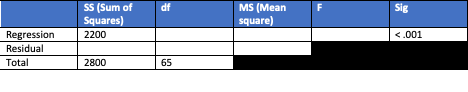
\includegraphics[width=1\linewidth]{img/ex_tab_lm} \caption{Invullen ANOVA tabel}\label{fig:extablm}
\end{figure}

\hypertarget{conclusies-1}{%
\section*{Conclusies}\label{conclusies-1}}


Enkele belangrijke stappen die je steeds moet doornemen:

\begin{itemize}
\tightlist
\item
  ANOVA-tabel en p-waarde
\item
  Determinatiecoëfficiënt (\(R^2\))
\item
  Voorwaarden vervuld (Lineariteit, onafhankelijk en residuen)
\item
  Residuenanalyse
\item
  Klinische relevantie!
\end{itemize}

\begin{itemize}
\tightlist
\item
  Regressie \(\neq\) een causaal verband.
\item
  Regressie is mogelijk met één of meerdere onafhankelijke variabelen.
\item
  De \(R^2\) zegt iets over hoe goed de regressielijn in staat is om \(Y\) te verklaren.
\item
  Regressie geeft steeds een lineair verband weer en is dus gerelateerd aan \(\rho\).
\item
  De afhankelijke variabele \(Y\) bij lieanire regressie is steeds continu.
\end{itemize}

\end{document}
